
\documentclass[11pt,a4paper]{article}

% ---------- Packages ----------
\usepackage[margin=1in]{geometry}
\usepackage{graphicx}
\usepackage{amsmath, amssymb, amsthm}
\usepackage{booktabs}
\usepackage{array}
\usepackage{enumitem}
\usepackage[hidelinks]{hyperref}
\usepackage{titlesec}

% Optional: tighter run-in paragraph/subparagraph spacing
\titlespacing*{\paragraph}{0pt}{1.25ex plus .5ex}{1em}
\titlespacing*{\subparagraph}{0pt}{1.0ex plus .5ex}{1em}

% ---------- Macros ----------
% Common Hamiltonian notation
\newcommand{\Hising}{H_{\mathrm{Ising}}}
\newcommand{\Htf}{H_{\mathrm{TF}}}
\newcommand{\Htot}{H=\Hising+\Htf}

% A small helper for nice math in tables
\newcommand{\NNZ}{\#\text{non-zero components}}

% Table column types
\newcolumntype{L}[1]{>{\raggedright\arraybackslash}p{#1}}
\newcolumntype{C}[1]{>{\centering\arraybackslash}p{#1}}

% ---------- Header ----------
\title{Scars of the Simple Ising Model on Discrete Geometries (Polyhedra)}
\author{}
\date{\today}

\begin{document}
\maketitle

% ============================================================
% OVERALL PARAGRAPH (global statement for the whole note)
% ============================================================
\section*{Introduction}
We are studying scars of the simple Ising model on discrete geometries (polyhedra). Here, \emph{scars} are identified as special, sparser eigenstates of the Hamiltonian which are simultaneously eigenstates of the Ising term and of the transverse-field (TF) term separately; in addition, each such state is annihilated by exactly one of the two terms.

\section*{Platonic Solids}
% ============================================================
% REPEAT THE BLOCK BELOW FOR EACH POLYHEDRON
% ============================================================

% -------------------- Polyhedron Block: START --------------------
\subsection*{Tetrahedron}

\subsubsection*{Overview and data.}
\begin{center}
  % Put your graphic at the very beginning of the subparagraph
  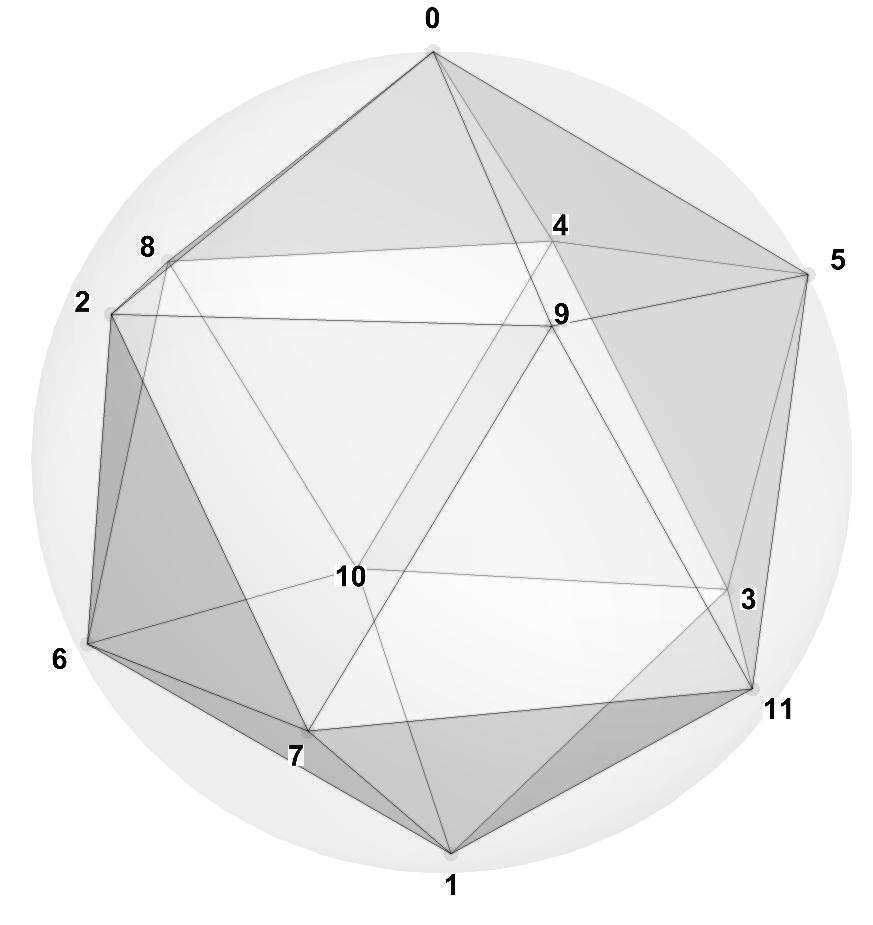
\includegraphics[width=.6\linewidth]{icosahedron}
\end{center}

\begin{itemize}[leftmargin=1.5em]
  \item \textbf{Duality / paired solid:} \texttt{<DUALITY or “self-dual”>}.
  \item \textbf{Vertices (V), Faces (F), Edges (E):} $V=\texttt{<V>}$,\; $F=\texttt{<F>}$,\; $E=\texttt{<E>}$.
  \item \textbf{Solid point group:} \texttt{<POINT-GROUP>}.\\
        \textbf{Vertex stabilizer subgroup:} \texttt{<STABILIZER>}.
  \item \textbf{Hamiltonian:} \(
        \Htot,\quad
        \dim\mathcal{H} = 2^{V}\ \text{(spin-$\tfrac12$ on each vertex).}
        \)
  \item \textbf{Eigenvalue range / normalization:} \texttt{<Specify conventions>}.
\end{itemize}

\subsubsection*{Scar structure: sets and multiplets.}
\begin{center}
  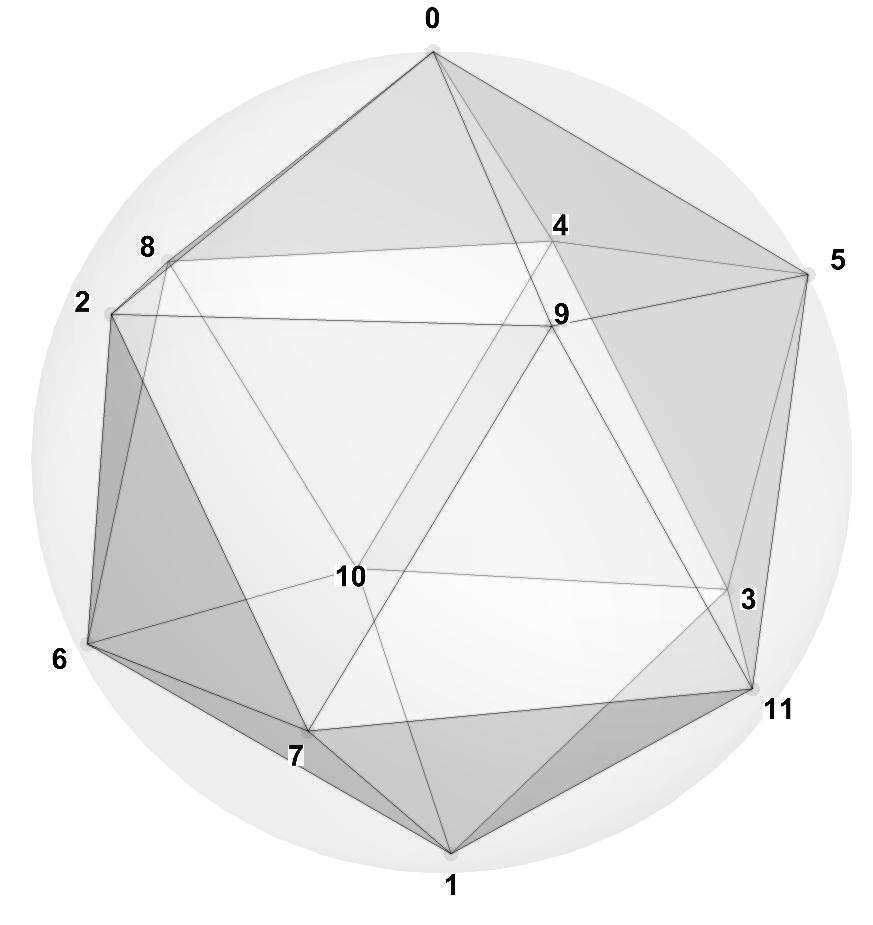
\includegraphics[width=.6\linewidth]{icosahedron}
\end{center}

\begin{itemize}[leftmargin=1.5em]
  \item \textbf{Number of scar sets:} \texttt{<1 or 2>}. 
  \item For each scar set $S_k$, fill one table per set:
\end{itemize}

\noindent\textit{Scar set} $S_{\texttt{<k>}}$:  
\begin{center}
\begin{tabular}{L{3.5cm} C{2.2cm} C{2.2cm} C{2.2cm} C{3.0cm} C{3.2cm}}
\toprule
\textbf{Multiplet label} & \textbf{Energy $E$} & \textbf{Degeneracy} & \textbf{Annihilated by} & \textbf{Non-zero components (vs.\ $2^{V}$)} \\
\midrule
\texttt{<m1>} & $\pm$ \texttt{<int>} & \texttt{<deg>} & \texttt{$\Hising$ / $\Htf$ / both} & \texttt{<\# non-zero> / $2^{\texttt{<V>}}$} \\
\bottomrule
\end{tabular}
\end{center}

\subsubsection*{Local properties (RDMs).}
\begin{center}
  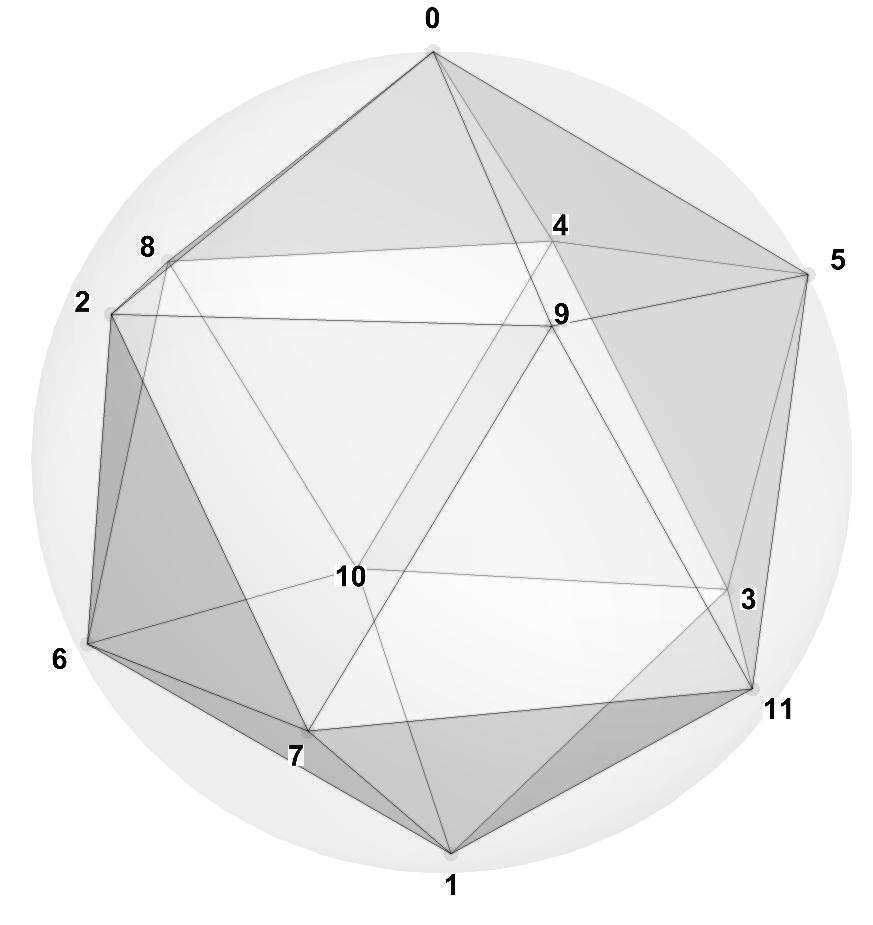
\includegraphics[width=.6\linewidth]{icosahedron}
\end{center}

\begin{itemize}[leftmargin=1.5em]
  \item \textbf{Local RDM definition:} $\rho_A=\mathrm{Tr}_{\bar A}(|\psi\rangle\langle\psi|)$ on compact subsets of $n=2,3,4,5,6$ sites, with $n < V/2$.
  \item \textbf{Compactness criterion:} \texttt{<how subsets chosen>}.
  \item \textbf{Diagnostics:} \texttt{<observables, entropies, purity, etc.>}.
\end{itemize}

% -------------------- Polyhedron Block: END --------------------

% -------------------- Polyhedron Block: START --------------------
\subsection*{Octahedron}

\subsubsection*{Overview and data.}
\begin{center}
  % Put your graphic at the very beginning of the subparagraph
  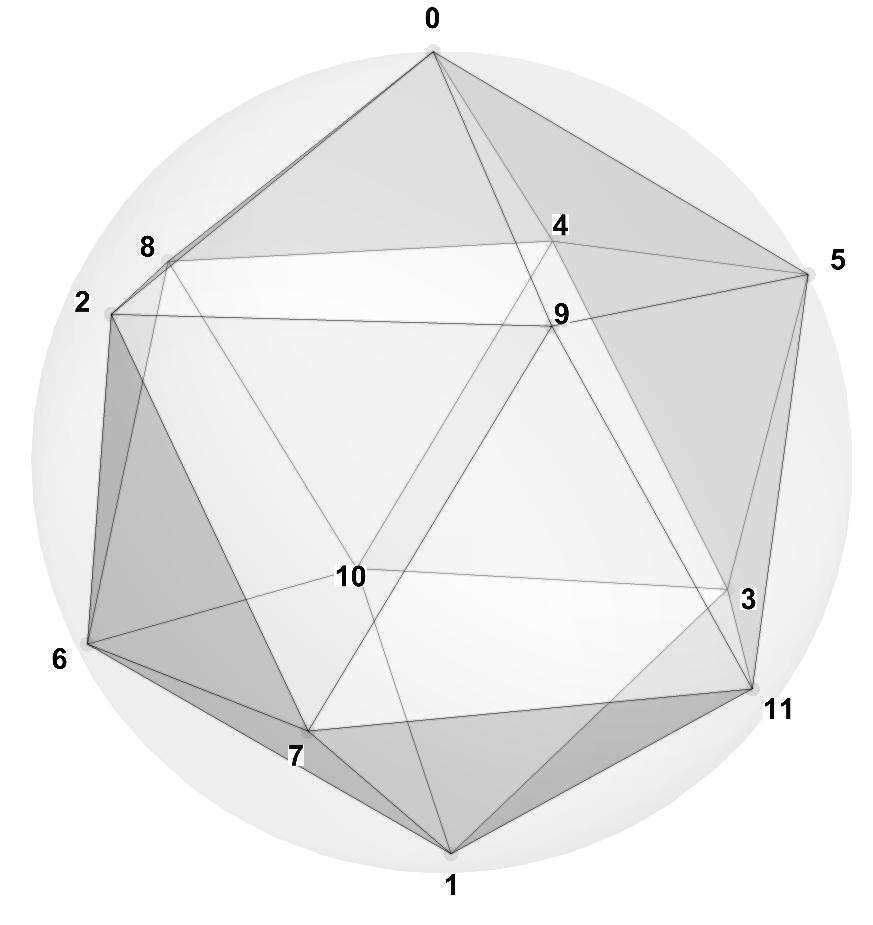
\includegraphics[width=.6\linewidth]{icosahedron}
\end{center}

\begin{itemize}[leftmargin=1.5em]
  \item \textbf{Duality / paired solid:} \texttt{<DUALITY or “self-dual”>}.
  \item \textbf{Vertices (V), Faces (F), Edges (E):} $V=\texttt{<V>}$,\; $F=\texttt{<F>}$,\; $E=\texttt{<E>}$.
  \item \textbf{Solid point group:} \texttt{<POINT-GROUP>}.\\
        \textbf{Vertex stabilizer subgroup:} \texttt{<STABILIZER>}.
  \item \textbf{Hamiltonian:} \(
        \Htot,\quad
        \dim\mathcal{H} = 2^{V}\ \text{(spin-$\tfrac12$ on each vertex).}
        \)
  \item \textbf{Eigenvalue range / normalization:} \texttt{<Specify conventions>}.
\end{itemize}

\subsubsection*{Scar structure: sets and multiplets.}
\begin{center}
  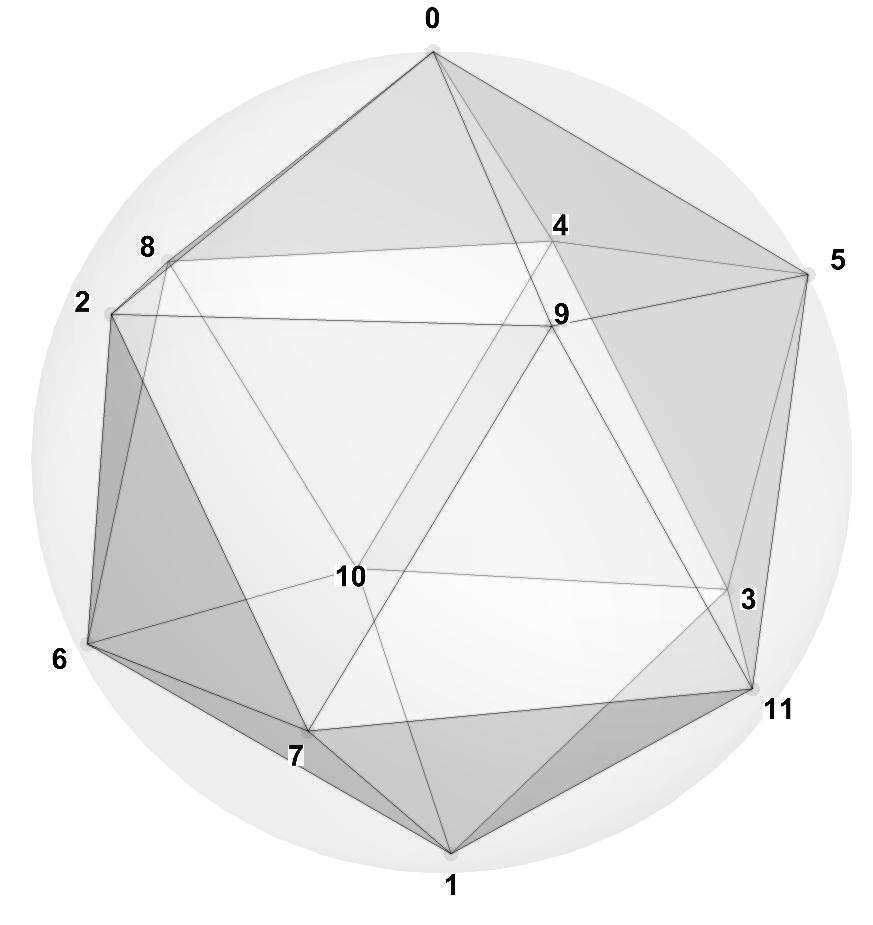
\includegraphics[width=.6\linewidth]{icosahedron}
\end{center}

\begin{itemize}[leftmargin=1.5em]
  \item \textbf{Number of scar sets:} \texttt{<1 or 2>}. 
  \item For each scar set $S_k$, fill one table per set:
\end{itemize}

\noindent\textit{Scar set} $S_{\texttt{<k>}}$:
\begin{center}
\begin{tabular}{L{3.5cm} C{2.2cm} C{2.2cm} C{2.2cm} C{3.0cm} C{3.2cm}}
\toprule
\textbf{Multiplet label} & \textbf{Energy $E$} & \textbf{Degeneracy} & \textbf{Annihilated by} & \textbf{Non-zero components (vs.\ $2^{V}$)} \\
\midrule
\texttt{<m1>} & $\pm$ \texttt{<int>} & \texttt{<deg> } &
\texttt{$\Hising$ / $\Htf$ / both} & \texttt{<\# non-zero> / $2^{\texttt{<V>}}$} \\
\bottomrule
\end{tabular}
\end{center}

\subsubsection*{Local properties (RDMs).}
\begin{center}
  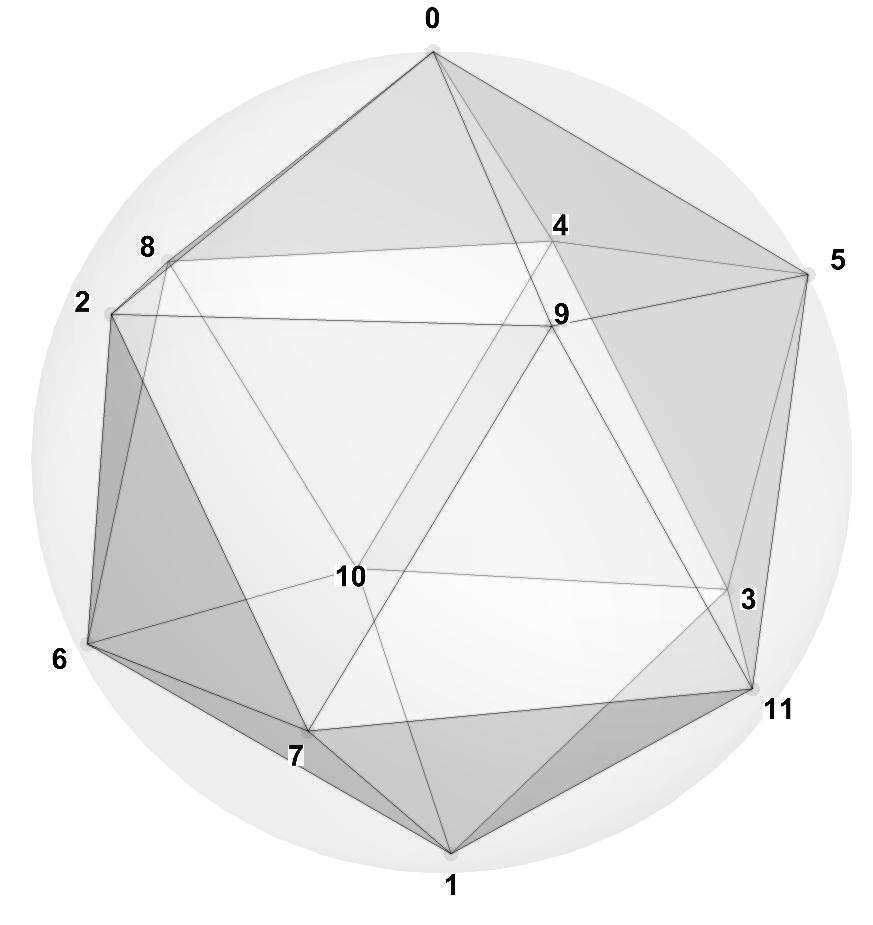
\includegraphics[width=.6\linewidth]{icosahedron}
\end{center}

\begin{itemize}[leftmargin=1.5em]
  \item \textbf{Local RDM definition:} $\rho_A=\mathrm{Tr}_{\bar A}(|\psi\rangle\langle\psi|)$ on compact subsets of $n=2,3,4,5,6$ sites, with $n < V/2$.
  \item \textbf{Compactness criterion:} \texttt{<how subsets chosen>}.
  \item \textbf{Diagnostics:} \texttt{<observables, entropies, purity, etc.>}.
\end{itemize}

% -------------------- Polyhedron Block: END --------------------

% -------------------- Polyhedron Block: START --------------------
\subsection*{Cube}

\subsubsection*{Overview and data.}
\begin{center}
  % Put your graphic at the very beginning of the subparagraph
  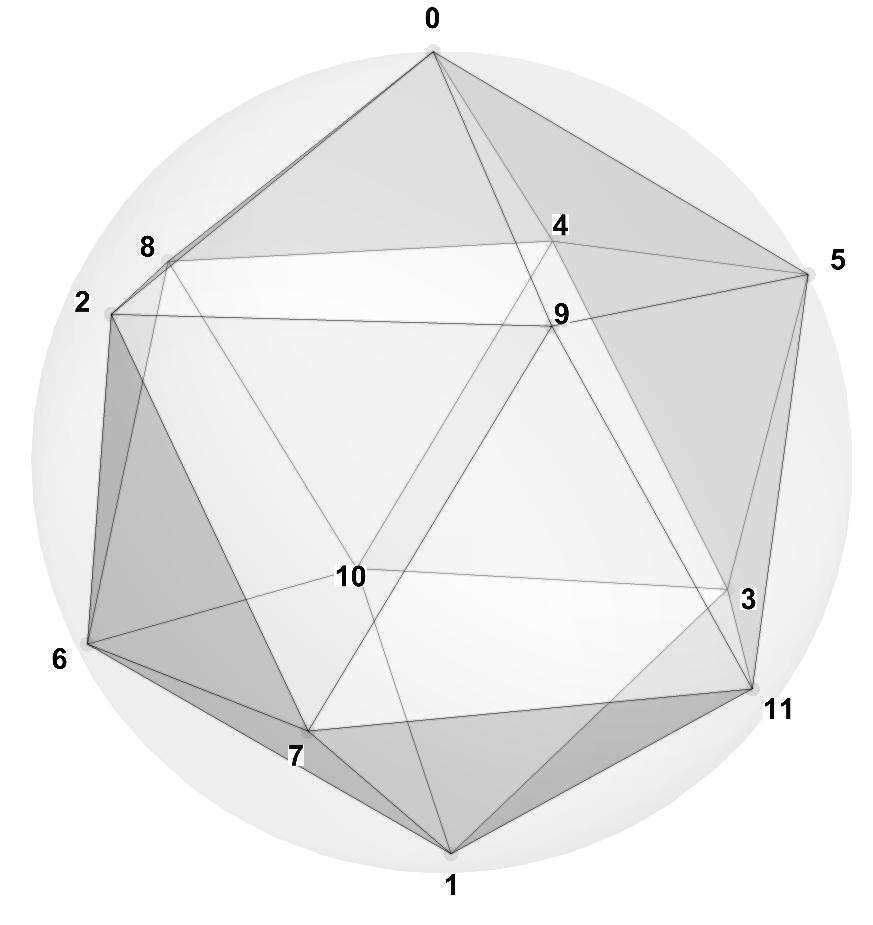
\includegraphics[width=.6\linewidth]{icosahedron}
\end{center}

\begin{itemize}[leftmargin=1.5em]
  \item \textbf{Duality / paired solid:} \texttt{<DUALITY or “self-dual”>}.
  \item \textbf{Vertices (V), Faces (F), Edges (E):} $V=\texttt{<V>}$,\; $F=\texttt{<F>}$,\; $E=\texttt{<E>}$.
  \item \textbf{Solid point group:} \texttt{<POINT-GROUP>}.\\
        \textbf{Vertex stabilizer subgroup:} \texttt{<STABILIZER>}.
  \item \textbf{Hamiltonian:} \(
        \Htot,\quad
        \dim\mathcal{H} = 2^{V}\ \text{(spin-$\tfrac12$ on each vertex).}
        \)
  \item \textbf{Eigenvalue range / normalization:} \texttt{<Specify conventions>}.
\end{itemize}

\subsubsection*{Scar structure: sets and multiplets.}
\begin{center}
  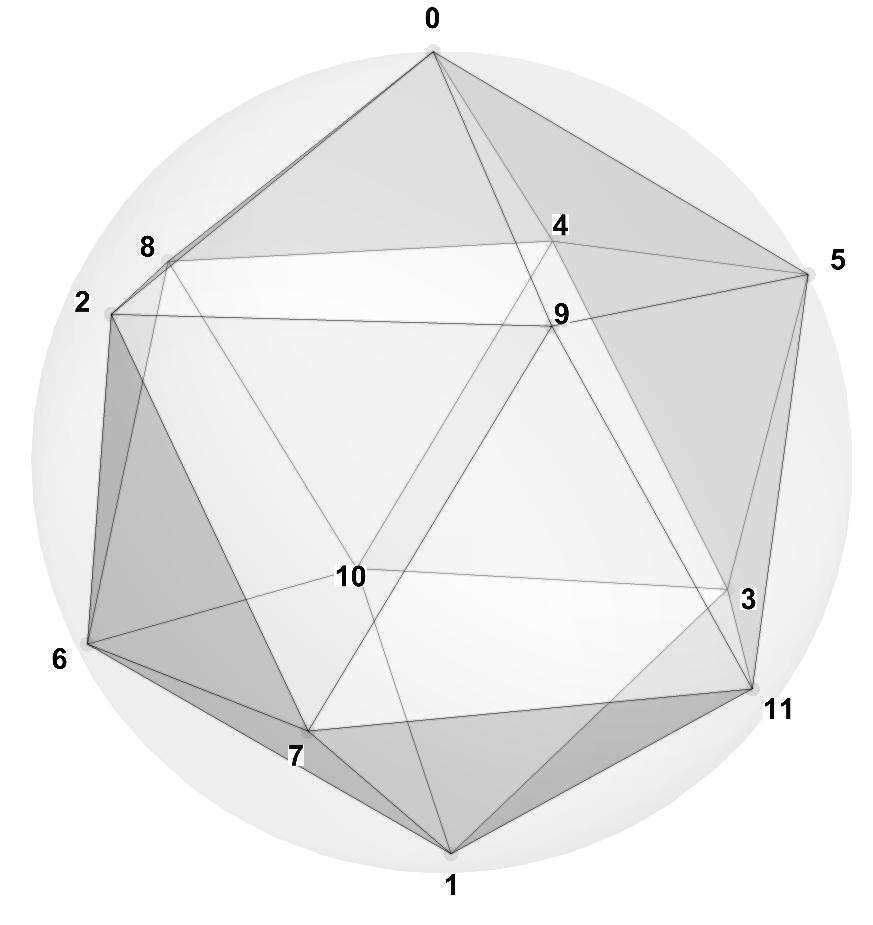
\includegraphics[width=.6\linewidth]{icosahedron}
\end{center}

\begin{itemize}[leftmargin=1.5em]
  \item \textbf{Number of scar sets:} \texttt{<1 or 2>}. 
  \item For each scar set $S_k$, fill one table per set:
\end{itemize}

\noindent\textit{Scar set} $S_{\texttt{<k>}}$:
\begin{center}
\begin{tabular}{L{3.5cm} C{2.2cm} C{2.2cm} C{2.2cm} C{3.0cm} C{3.2cm}}
\toprule
\textbf{Multiplet label} & \textbf{Energy $E$} & \textbf{Degeneracy} & \textbf{Annihilated by} & \textbf{Non-zero components (vs.\ $2^{V}$)} \\
\midrule
\texttt{<m1>} & $\pm$ \texttt{<int>}  & \texttt{<deg> } &
\texttt{$\Hising$ / $\Htf$ / both} & \texttt{<\# non-zero> / $2^{\texttt{<V>}}$} \\
\bottomrule
\end{tabular}
\end{center}

\subsubsection*{Local properties (RDMs).}
\begin{center}
  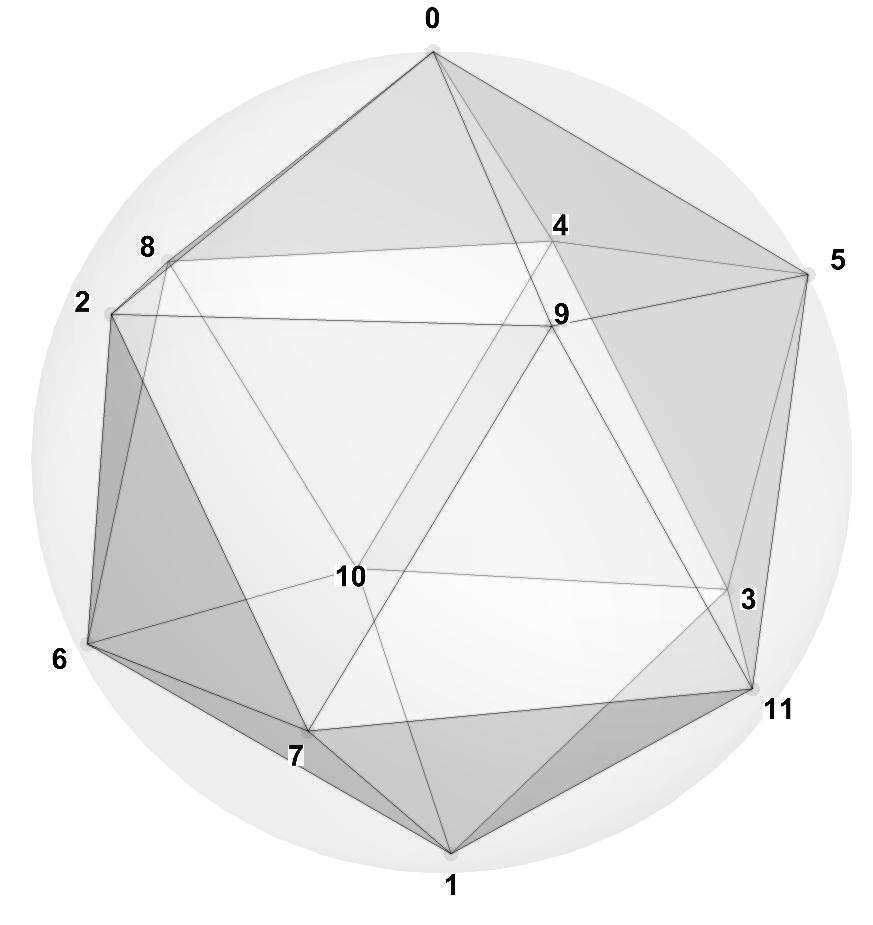
\includegraphics[width=.6\linewidth]{icosahedron}
\end{center}

\begin{itemize}[leftmargin=1.5em]
  \item \textbf{Local RDM definition:} $\rho_A=\mathrm{Tr}_{\bar A}(|\psi\rangle\langle\psi|)$ on compact subsets of $n=2,3,4,5,6$ sites, with $n < V/2$.
  \item \textbf{Compactness criterion:} \texttt{<how subsets chosen>}.
  \item \textbf{Diagnostics:} \texttt{<observables, entropies, purity, etc.>}.
\end{itemize}

% -------------------- Polyhedron Block: END --------------------

% -------------------- Polyhedron Block: START --------------------
\subsection*{Icosahedron}

\subsubsection*{Overview and data.}
\begin{center}
  % Put your graphic at the very beginning of the subparagraph
  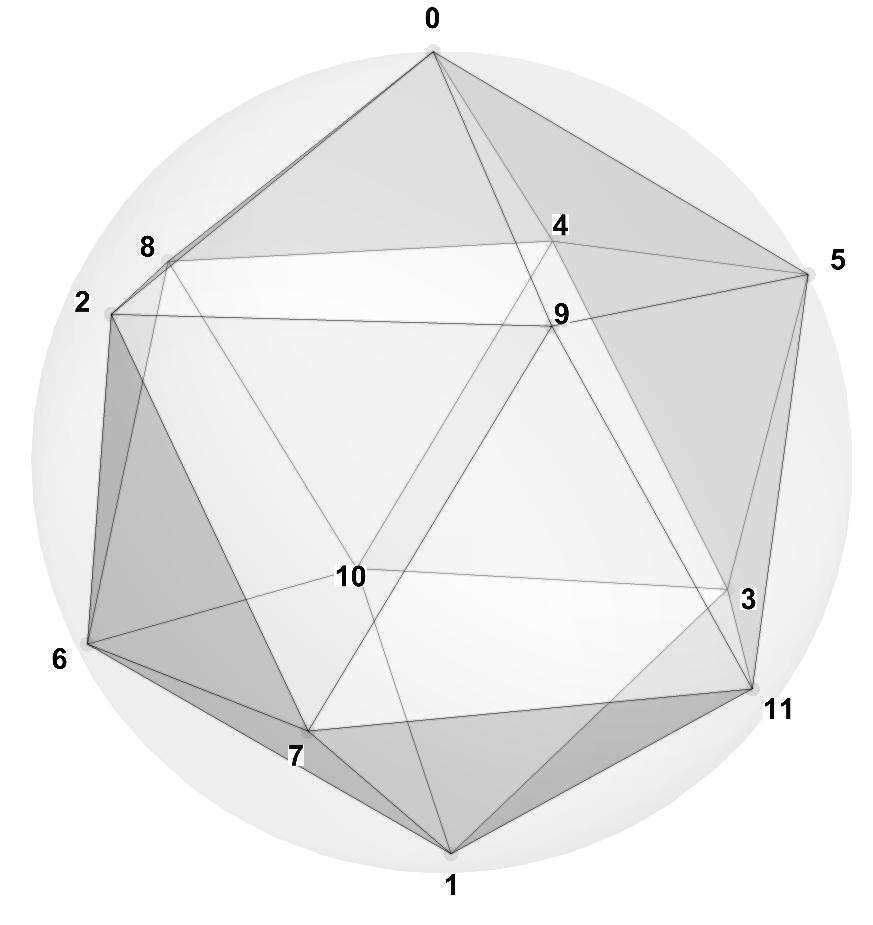
\includegraphics[width=.6\linewidth]{icosahedron}
\end{center}

\begin{itemize}[leftmargin=1.5em]
  \item \textbf{Duality / paired solid:} \texttt{<DUALITY or “self-dual”>}.
  \item \textbf{Vertices (V), Faces (F), Edges (E):} $V=\texttt{<V>}$,\; $F=\texttt{<F>}$,\; $E=\texttt{<E>}$.
  \item \textbf{Solid point group:} \texttt{<POINT-GROUP>}.\\
        \textbf{Vertex stabilizer subgroup:} \texttt{<STABILIZER>}.
  \item \textbf{Hamiltonian:} \(
        \Htot,\quad
        \dim\mathcal{H} = 2^{V}\ \text{(spin-$\tfrac12$ on each vertex).}
        \)
  \item \textbf{Eigenvalue range / normalization:} \texttt{<Specify conventions>}.
\end{itemize}

\subsubsection*{Scar structure: sets and multiplets.}
\begin{center}
  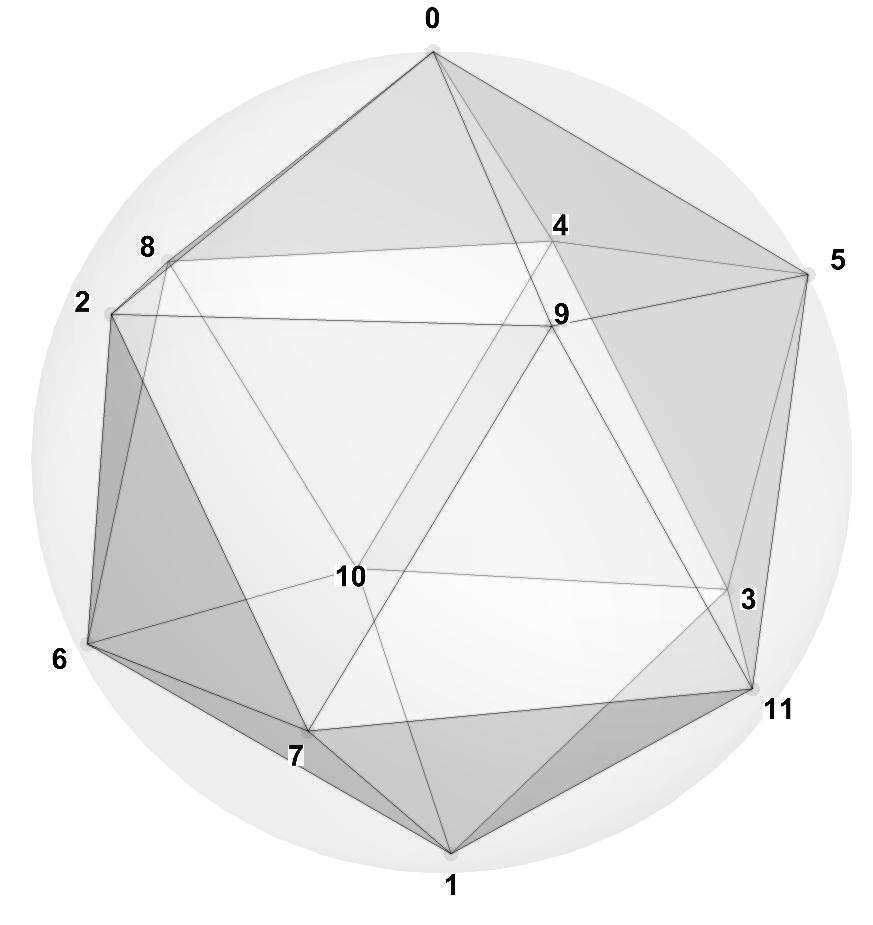
\includegraphics[width=.6\linewidth]{icosahedron}
\end{center}

\begin{itemize}[leftmargin=1.5em]
  \item \textbf{Number of scar sets:} \texttt{<1 or 2>}. 
  \item For each scar set $S_k$, fill one table per set:
\end{itemize}

\noindent\textit{Scar set} $S_{\texttt{<k>}}$:
\begin{center}
\begin{tabular}{L{3.5cm} C{2.2cm} C{2.2cm} C{2.2cm} C{3.0cm} C{3.2cm}}
\toprule
\textbf{Multiplet label} & \textbf{Energy $E$} & \textbf{Degeneracy} & \textbf{Annihilated by} & \textbf{Non-zero components (vs.\ $2^{V}$)} \\
\midrule
\texttt{<m1>} & $\pm$ \texttt{<int>}  & \texttt{<deg> } &
\texttt{$\Hising$ / $\Htf$ / both} & \texttt{<\# non-zero> / $2^{\texttt{<V>}}$} \\
\bottomrule
\end{tabular}
\end{center}

\subsubsection*{Local properties (RDMs).}
\begin{center}
  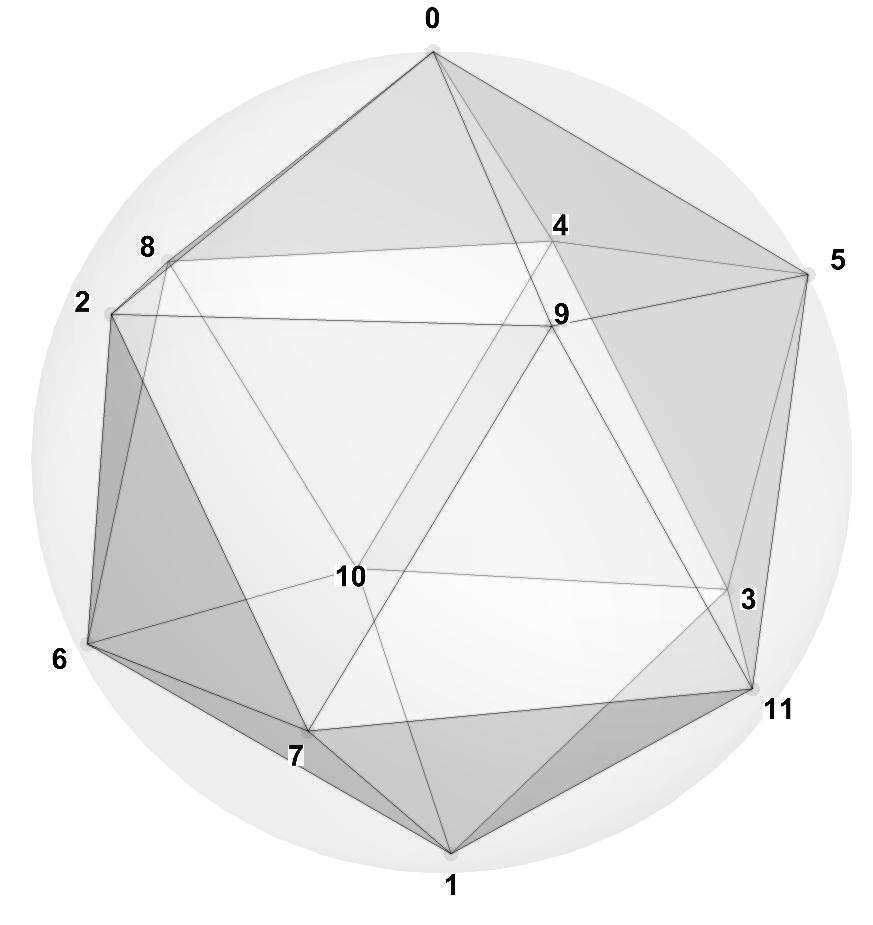
\includegraphics[width=.6\linewidth]{icosahedron}
\end{center}

\begin{itemize}[leftmargin=1.5em]
  \item \textbf{Local RDM definition:} $\rho_A=\mathrm{Tr}_{\bar A}(|\psi\rangle\langle\psi|)$ on compact subsets of $n=2,3,4,5,6$ sites, with $n < V/2$.
  \item \textbf{Compactness criterion:} \texttt{<how subsets chosen>}.
  \item \textbf{Diagnostics:} \texttt{<observables, entropies, purity, etc.>}.
\end{itemize}

% -------------------- Polyhedron Block: END --------------------

% -------------------- Polyhedron Block: START --------------------
\subsection*{Dodecahedron}

\subsubsection*{Overview and data.}
\begin{center}
  % Put your graphic at the very beginning of the subparagraph
  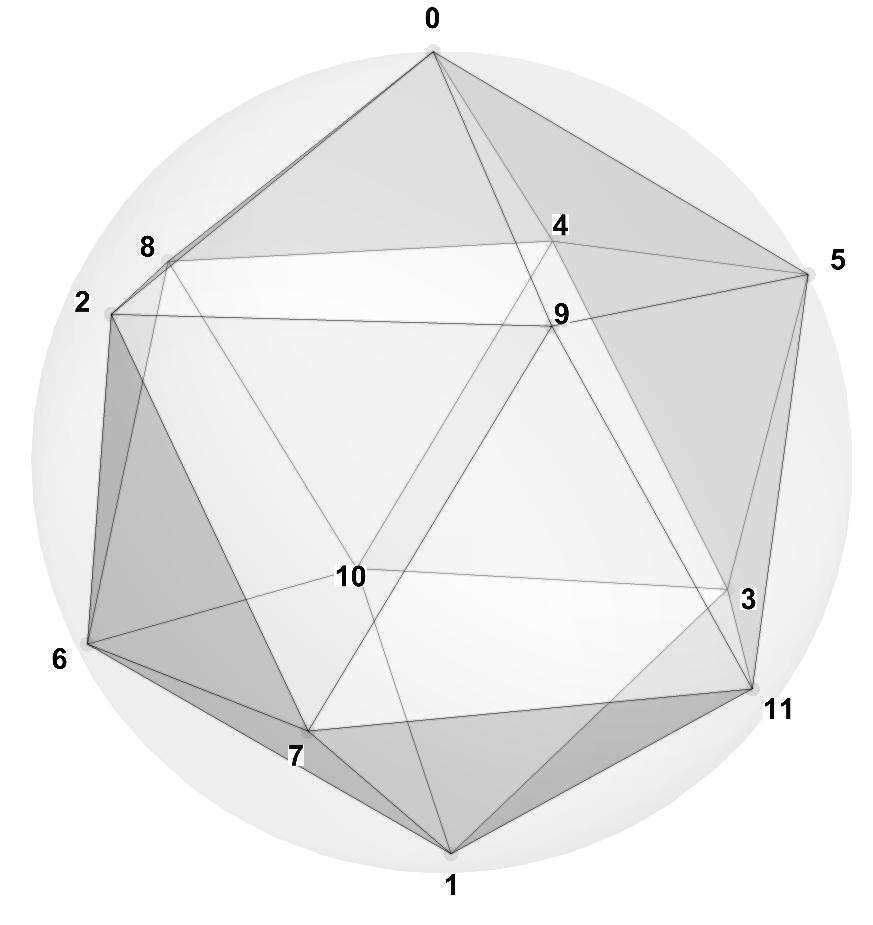
\includegraphics[width=.6\linewidth]{icosahedron}
\end{center}

\begin{itemize}[leftmargin=1.5em]
  \item \textbf{Duality / paired solid:} \texttt{<DUALITY or “self-dual”>}.
  \item \textbf{Vertices (V), Faces (F), Edges (E):} $V=\texttt{<V>}$,\; $F=\texttt{<F>}$,\; $E=\texttt{<E>}$.
  \item \textbf{Solid point group:} \texttt{<POINT-GROUP>}.\\
        \textbf{Vertex stabilizer subgroup:} \texttt{<STABILIZER>}.
  \item \textbf{Hamiltonian:} \(
        \Htot,\quad
        \dim\mathcal{H} = 2^{V}\ \text{(spin-$\tfrac12$ on each vertex).}
        \)
  \item \textbf{Eigenvalue range / normalization:} \texttt{<Specify conventions>}.
\end{itemize}

\subsubsection*{Scar structure: sets and multiplets.}
\begin{center}
  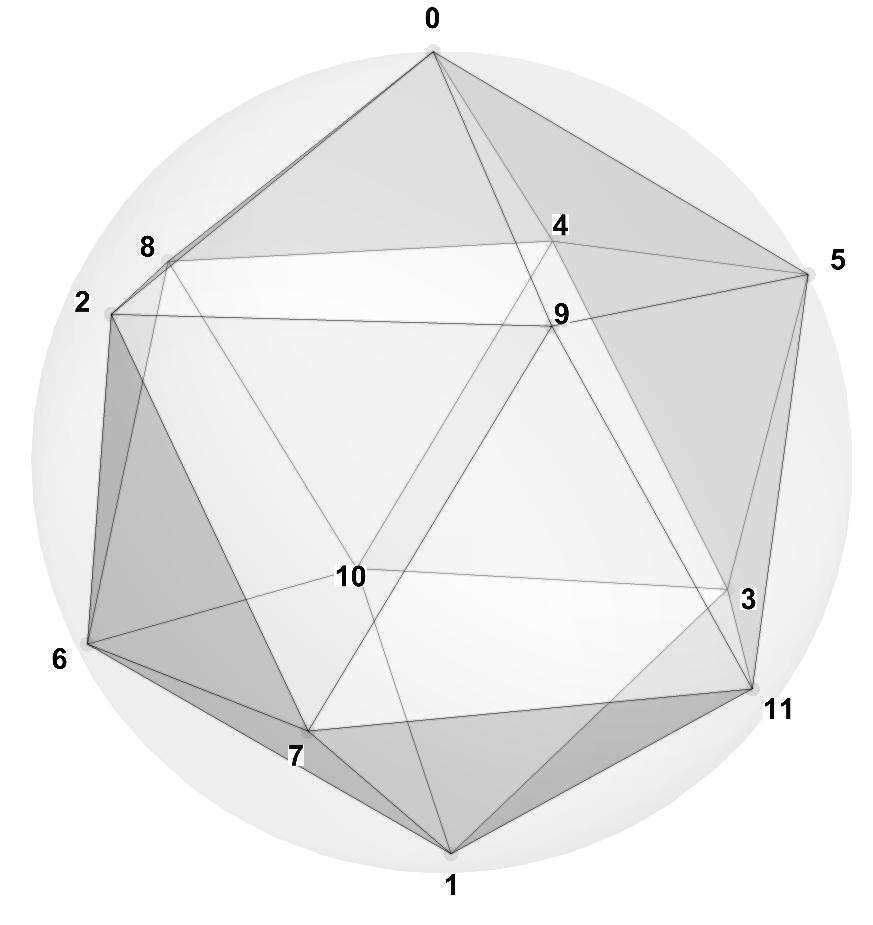
\includegraphics[width=.6\linewidth]{icosahedron}
\end{center}

\begin{itemize}[leftmargin=1.5em]
  \item \textbf{Number of scar sets:} \texttt{<1 or 2>}. 
  \item For each scar set $S_k$, fill one table per set:
\end{itemize}

\noindent\textit{Scar set} $S_{\texttt{<k>}}$:
\begin{center}
\begin{tabular}{L{3.5cm} C{2.2cm} C{2.2cm} C{2.2cm} C{3.0cm} C{3.2cm}}
\toprule
\textbf{Multiplet label} & \textbf{Energy $E$} & \textbf{Degeneracy} & \textbf{Annihilated by} & \textbf{Non-zero components (vs.\ $2^{V}$)} \\
\midrule
\texttt{<m1>} & $\pm$ \texttt{<int>} & \texttt{<deg> } &
\texttt{$\Hising$ / $\Htf$ / both} & \texttt{<\# non-zero> / $2^{\texttt{<V>}}$} \\
\bottomrule
\end{tabular}
\end{center}

\subsubsection*{Local properties (RDMs).}
\begin{center}
  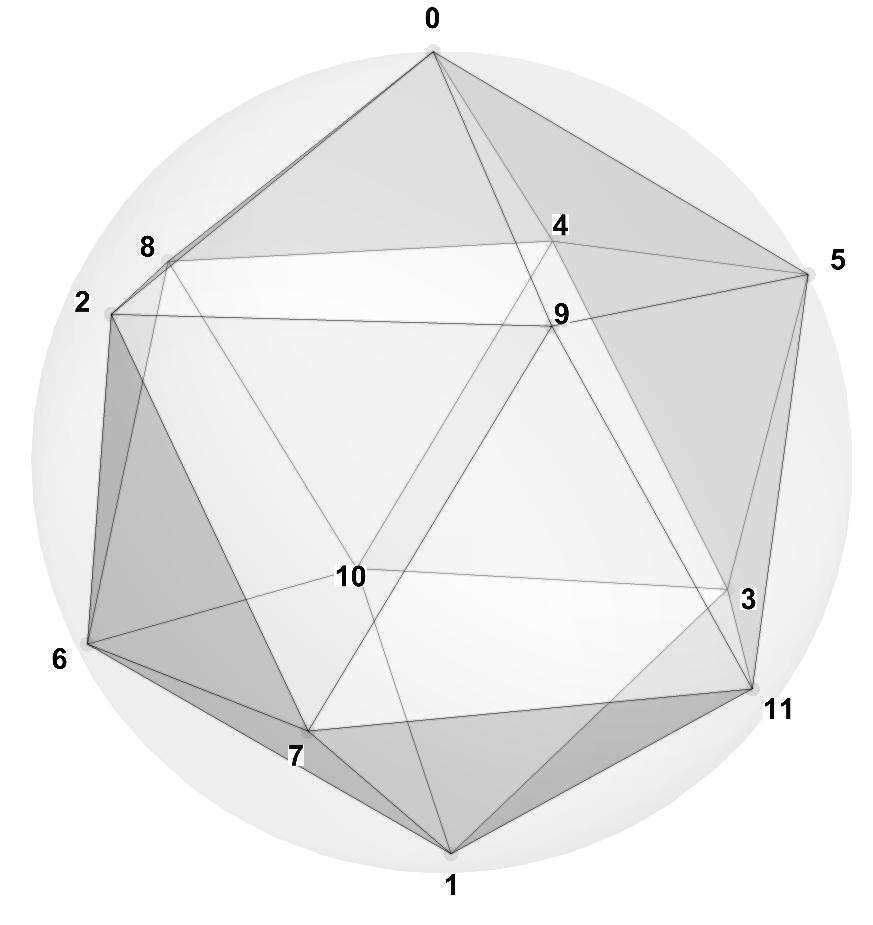
\includegraphics[width=.6\linewidth]{icosahedron}
\end{center}

\begin{itemize}[leftmargin=1.5em]
  \item \textbf{Local RDM definition:} $\rho_A=\mathrm{Tr}_{\bar A}(|\psi\rangle\langle\psi|)$ on compact subsets of $n=2,3,4,5,6$ sites, with $n < V/2$.
  \item \textbf{Compactness criterion:} \texttt{<how subsets chosen>}.
  \item \textbf{Diagnostics:} \texttt{<observables, entropies, purity, etc.>}.
\end{itemize}

% -------------------- Polyhedron Block: END --------------------

\section*{Catalan Solids}
% ============================================================
% REPEAT THE BLOCK BELOW FOR EACH POLYHEDRON
% ============================================================

% -------------------- Polyhedron Block: START --------------------
\subsection*{Triakis Tetrahedron}

\subsubsection*{Overview and data.}
\begin{center}
  % Put your graphic at the very beginning of the subparagraph
  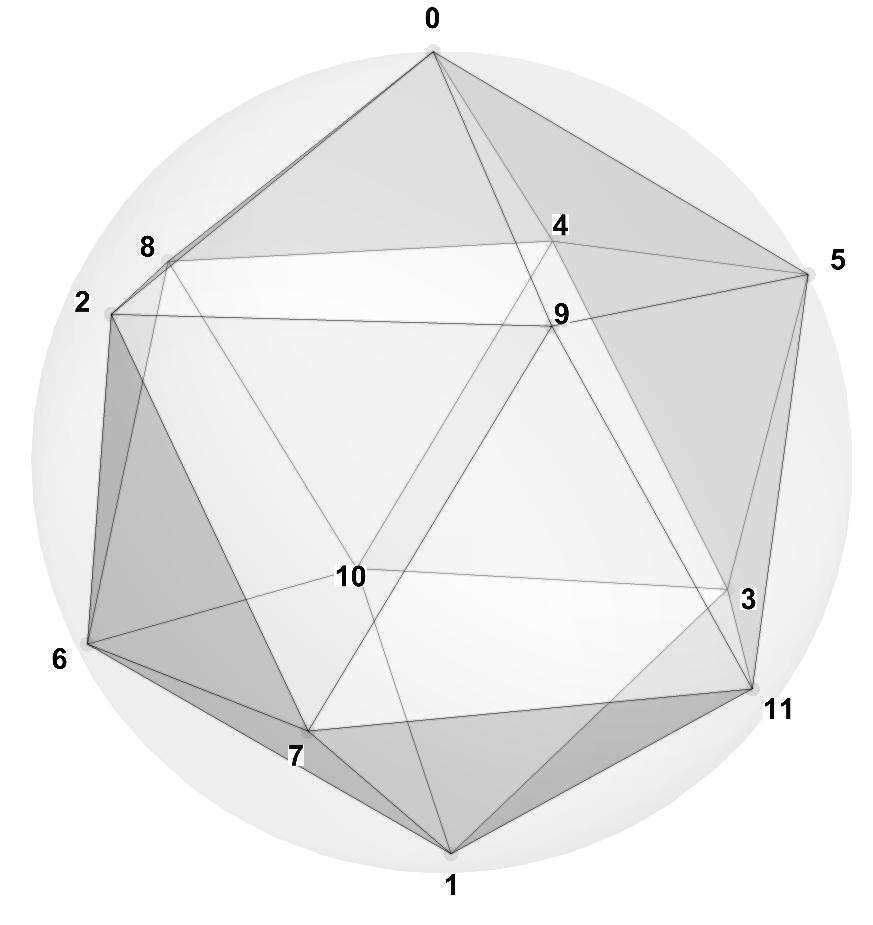
\includegraphics[width=.6\linewidth]{icosahedron}
\end{center}

\begin{itemize}[leftmargin=1.5em]
  \item \textbf{Duality / paired solid:} \texttt{<DUALITY or “self-dual”>}.
  \item \textbf{Vertices (V), Faces (F), Edges (E):} $V=\texttt{<V>}$,\; $F=\texttt{<F>}$,\; $E=\texttt{<E>}$.
  \item \textbf{Solid point group:} \texttt{<POINT-GROUP>}.\\
        \textbf{Vertex stabilizer subgroup:} \texttt{<STABILIZER>}.
  \item \textbf{Hamiltonian:} \(
        \Htot,\quad
        \dim\mathcal{H} = 2^{V}\ \text{(spin-$\tfrac12$ on each vertex).}
        \)
  \item \textbf{Eigenvalue range / normalization:} \texttt{<Specify conventions>}.
\end{itemize}

\subsubsection*{Scar structure: sets and multiplets.}
\begin{center}
  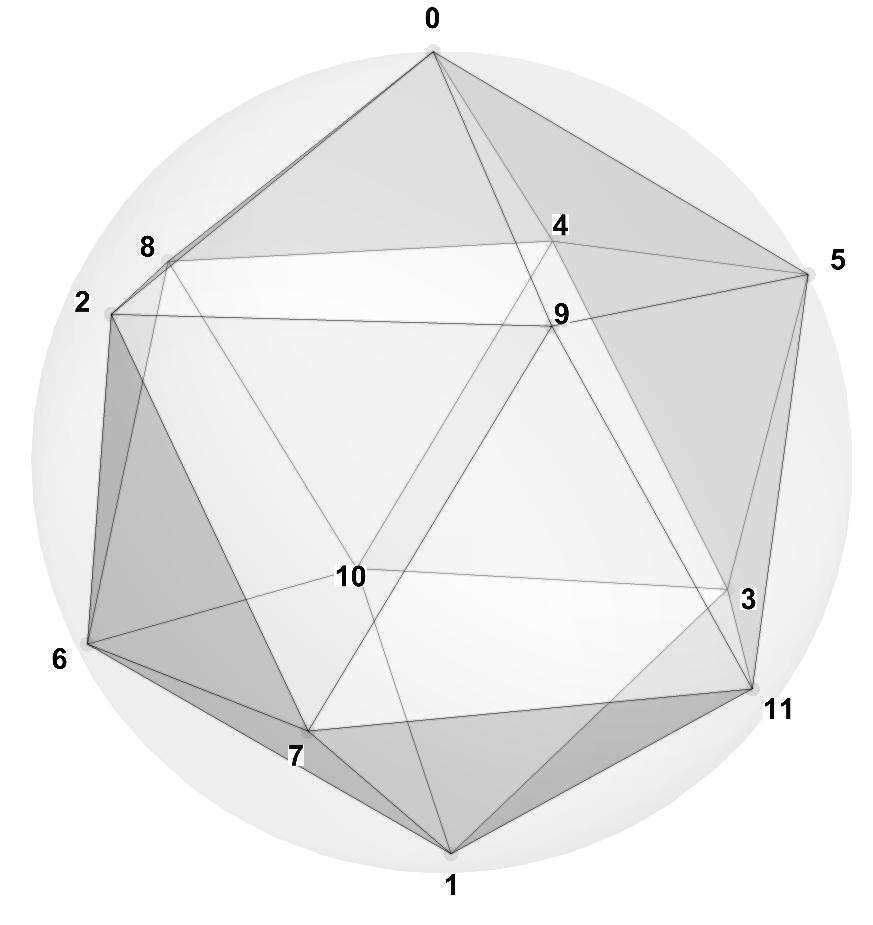
\includegraphics[width=.6\linewidth]{icosahedron}
\end{center}

\begin{itemize}[leftmargin=1.5em]
  \item \textbf{Number of scar sets:} \texttt{<1 or 2>}. 
  \item For each scar set $S_k$, fill one table per set:
\end{itemize}

\noindent\textit{Scar set} $S_{\texttt{<k>}}$:
\begin{center}
\begin{tabular}{L{3.5cm} C{2.2cm} C{2.2cm} C{2.2cm} C{3.0cm} C{3.2cm}}
\toprule
\textbf{Multiplet label} & \textbf{Energy $E$} & \textbf{Degeneracy} & \textbf{Annihilated by} & \textbf{Non-zero components (vs.\ $2^{V}$)} \\
\midrule
\texttt{<m1>} & $\pm$ \texttt{<int>} & \texttt{<deg> } &
\texttt{$\Hising$ / $\Htf$ / both} & \texttt{<\# non-zero> / $2^{\texttt{<V>}}$} \\
\bottomrule
\end{tabular}
\end{center}

\subsubsection*{Local properties (RDMs).}
\begin{center}
  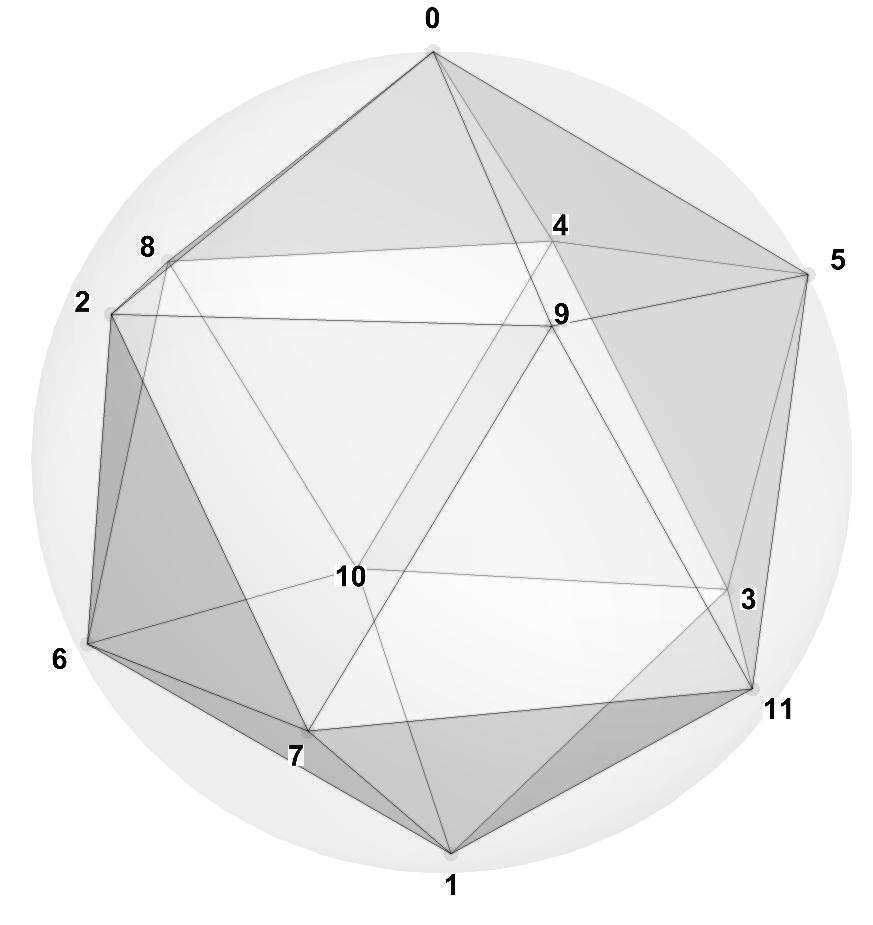
\includegraphics[width=.6\linewidth]{icosahedron}
\end{center}

\begin{itemize}[leftmargin=1.5em]
  \item \textbf{Local RDM definition:} $\rho_A=\mathrm{Tr}_{\bar A}(|\psi\rangle\langle\psi|)$ on compact subsets of $n=2,3,4,5,6$ sites, with $n < V/2$.
  \item \textbf{Compactness criterion:} \texttt{<how subsets chosen>}.
  \item \textbf{Diagnostics:} \texttt{<observables, entropies, purity, etc.>}.
\end{itemize}

% -------------------- Polyhedron Block: END --------------------

% -------------------- Polyhedron Block: START --------------------
\subsection*{Rhombic Dodecahedron}

\subsubsection*{Overview and data.}
\begin{center}
  % Put your graphic at the very beginning of the subparagraph
  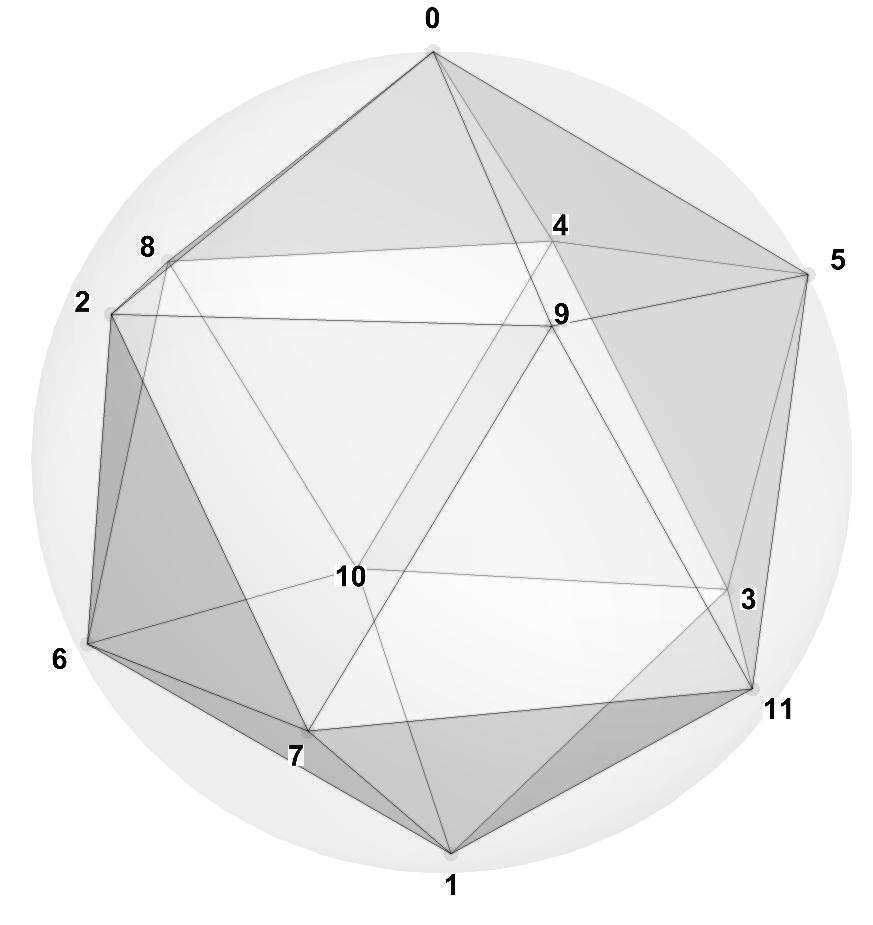
\includegraphics[width=.6\linewidth]{icosahedron}
\end{center}

\begin{itemize}[leftmargin=1.5em]
  \item \textbf{Duality / paired solid:} \texttt{<DUALITY or “self-dual”>}.
  \item \textbf{Vertices (V), Faces (F), Edges (E):} $V=\texttt{<V>}$,\; $F=\texttt{<F>}$,\; $E=\texttt{<E>}$.
  \item \textbf{Solid point group:} \texttt{<POINT-GROUP>}.\\
        \textbf{Vertex stabilizer subgroup:} \texttt{<STABILIZER>}.
  \item \textbf{Hamiltonian:} \(
        \Htot,\quad
        \dim\mathcal{H} = 2^{V}\ \text{(spin-$\tfrac12$ on each vertex).}
        \)
  \item \textbf{Eigenvalue range / normalization:} \texttt{<Specify conventions>}.
\end{itemize}

\subsubsection*{Scar structure: sets and multiplets.}
\begin{center}
  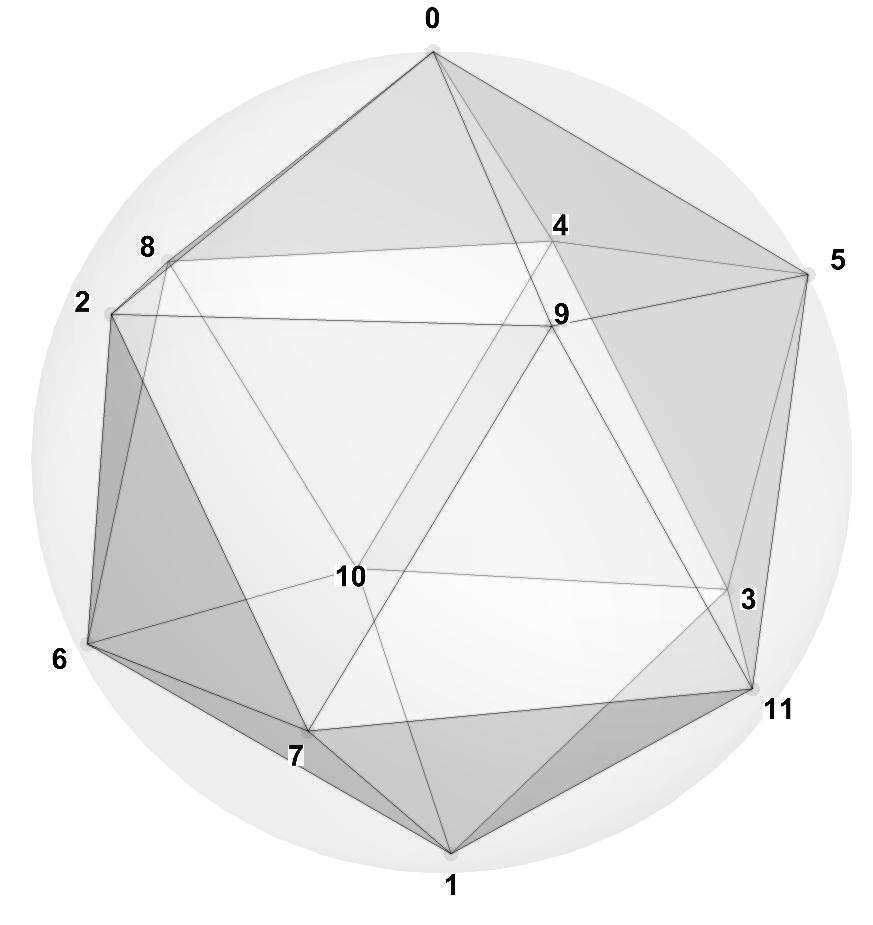
\includegraphics[width=.6\linewidth]{icosahedron}
\end{center}

\begin{itemize}[leftmargin=1.5em]
  \item \textbf{Number of scar sets:} \texttt{<1 or 2>}. 
  \item For each scar set $S_k$, fill one table per set:
\end{itemize}

\noindent\textit{Scar set} $S_{\texttt{<k>}}$:
\begin{center}
\begin{tabular}{L{3.5cm} C{2.2cm} C{2.2cm} C{2.2cm} C{3.0cm} C{3.2cm}}
\toprule
\textbf{Multiplet label} & \textbf{Energy $E$} & \textbf{Degeneracy} & \textbf{Annihilated by} & \textbf{Non-zero components (vs.\ $2^{V}$)} \\
\midrule
\texttt{<m1>} & $\pm$ \texttt{<int>} & \texttt{<deg> } &
\texttt{$\Hising$ / $\Htf$ / both} & \texttt{<\# non-zero> / $2^{\texttt{<V>}}$} \\
\bottomrule
\end{tabular}
\end{center}

\subsubsection*{Local properties (RDMs).}
\begin{center}
  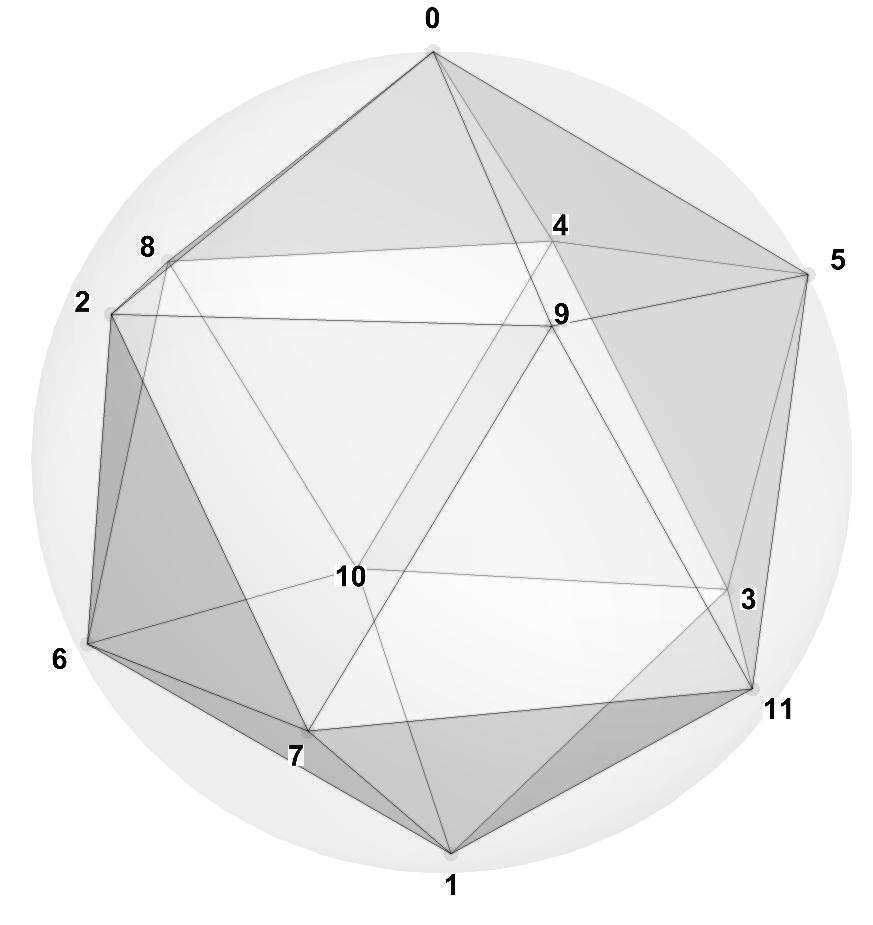
\includegraphics[width=.6\linewidth]{icosahedron}
\end{center}

\begin{itemize}[leftmargin=1.5em]
  \item \textbf{Local RDM definition:} $\rho_A=\mathrm{Tr}_{\bar A}(|\psi\rangle\langle\psi|)$ on compact subsets of $n=2,3,4,5,6$ sites, with $n < V/2$.
  \item \textbf{Compactness criterion:} \texttt{<how subsets chosen>}.
  \item \textbf{Diagnostics:} \texttt{<observables, entropies, purity, etc.>}.
\end{itemize}

% -------------------- Polyhedron Block: END --------------------

% -------------------- Polyhedron Block: START --------------------
\subsection*{Triakis Octahedron}

\subsubsection*{Overview and data.}
\begin{center}
  % Put your graphic at the very beginning of the subparagraph
  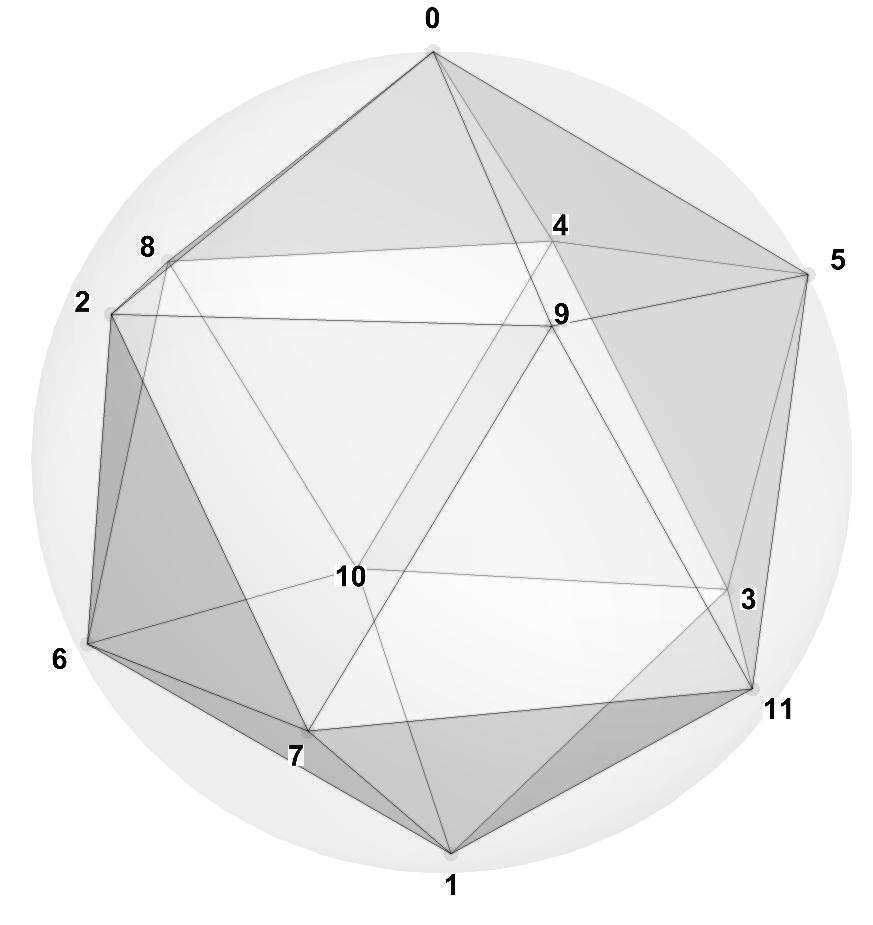
\includegraphics[width=.6\linewidth]{icosahedron}
\end{center}

\begin{itemize}[leftmargin=1.5em]
  \item \textbf{Duality / paired solid:} \texttt{<DUALITY or “self-dual”>}.
  \item \textbf{Vertices (V), Faces (F), Edges (E):} $V=\texttt{<V>}$,\; $F=\texttt{<F>}$,\; $E=\texttt{<E>}$.
  \item \textbf{Solid point group:} \texttt{<POINT-GROUP>}.\\
        \textbf{Vertex stabilizer subgroup:} \texttt{<STABILIZER>}.
  \item \textbf{Hamiltonian:} \(
        \Htot,\quad
        \dim\mathcal{H} = 2^{V}\ \text{(spin-$\tfrac12$ on each vertex).}
        \)
  \item \textbf{Eigenvalue range / normalization:} \texttt{<Specify conventions>}.
\end{itemize}

\subsubsection*{Scar structure: sets and multiplets.}
\begin{center}
  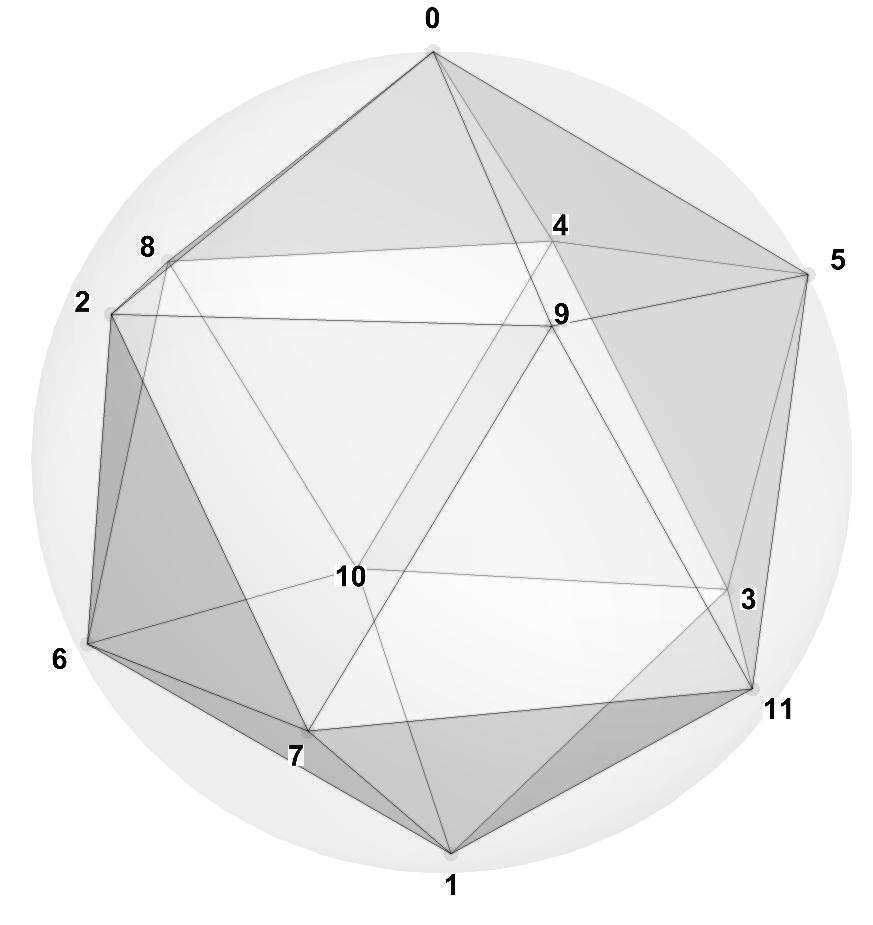
\includegraphics[width=.6\linewidth]{icosahedron}
\end{center}

\begin{itemize}[leftmargin=1.5em]
  \item \textbf{Number of scar sets:} \texttt{<1 or 2>}. 
  \item For each scar set $S_k$, fill one table per set:
\end{itemize}

\noindent\textit{Scar set} $S_{\texttt{<k>}}$:
\begin{center}
\begin{tabular}{L{3.5cm} C{2.2cm} C{2.2cm} C{2.2cm} C{3.0cm} C{3.2cm}}
\toprule
\textbf{Multiplet label} & \textbf{Energy $E$} & \textbf{Degeneracy} & \textbf{Annihilated by} & \textbf{Non-zero components (vs.\ $2^{V}$)} \\
\midrule
\texttt{<m1>} & $\pm$ \texttt{<int>} & \texttt{<deg> } &
\texttt{$\Hising$ / $\Htf$ / both} & \texttt{<\# non-zero> / $2^{\texttt{<V>}}$} \\
\bottomrule
\end{tabular}
\end{center}

\subsubsection*{Local properties (RDMs).}
\begin{center}
  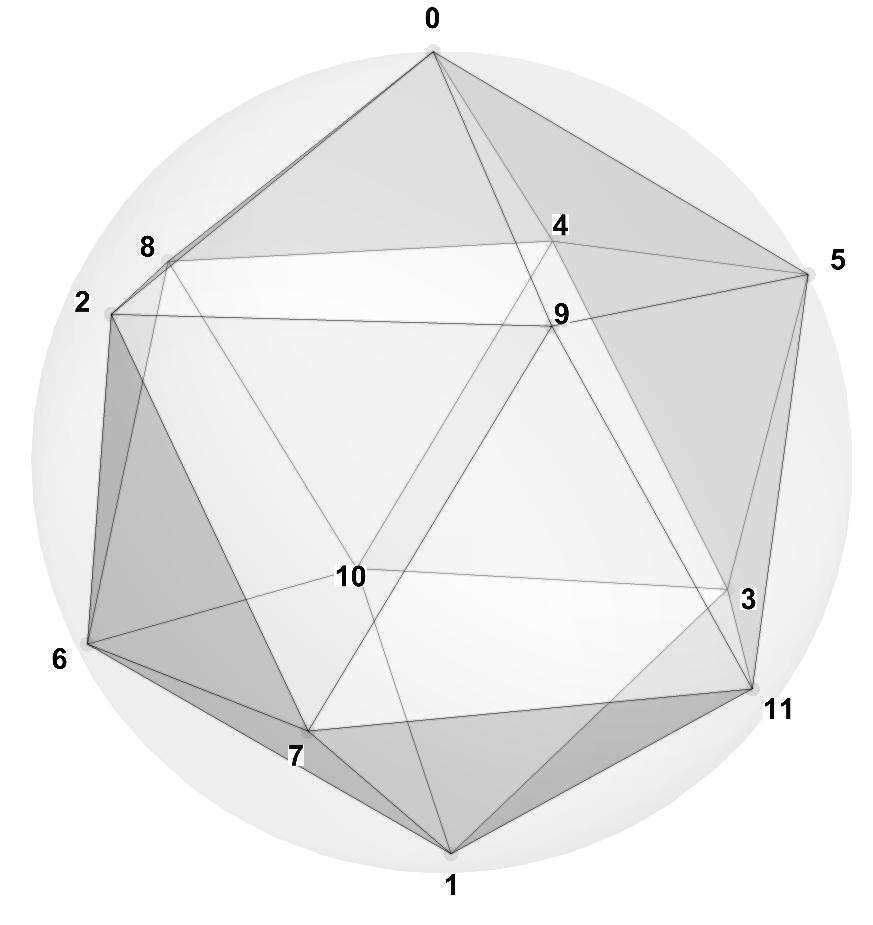
\includegraphics[width=.6\linewidth]{icosahedron}
\end{center}

\begin{itemize}[leftmargin=1.5em]
  \item \textbf{Local RDM definition:} $\rho_A=\mathrm{Tr}_{\bar A}(|\psi\rangle\langle\psi|)$ on compact subsets of $n=2,3,4,5,6$ sites, with $n < V/2$.
  \item \textbf{Compactness criterion:} \texttt{<how subsets chosen>}.
  \item \textbf{Diagnostics:} \texttt{<observables, entropies, purity, etc.>}.
\end{itemize}

% -------------------- Polyhedron Block: END --------------------

% -------------------- Polyhedron Block: START --------------------
\subsection*{Tetrakis Hexahedron}

\subsubsection*{Overview and data.}
\begin{center}
  % Put your graphic at the very beginning of the subparagraph
  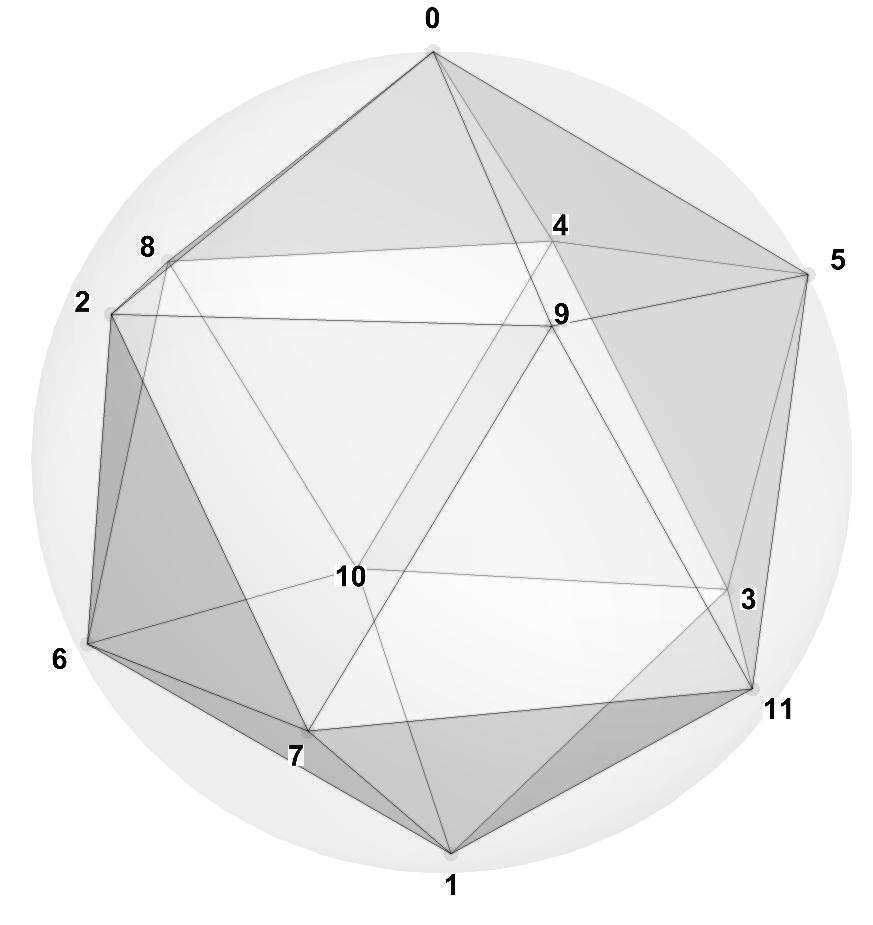
\includegraphics[width=.6\linewidth]{icosahedron}
\end{center}

\begin{itemize}[leftmargin=1.5em]
  \item \textbf{Duality / paired solid:} \texttt{<DUALITY or “self-dual”>}.
  \item \textbf{Vertices (V), Faces (F), Edges (E):} $V=\texttt{<V>}$,\; $F=\texttt{<F>}$,\; $E=\texttt{<E>}$.
  \item \textbf{Solid point group:} \texttt{<POINT-GROUP>}.\\
        \textbf{Vertex stabilizer subgroup:} \texttt{<STABILIZER>}.
  \item \textbf{Hamiltonian:} \(
        \Htot,\quad
        \dim\mathcal{H} = 2^{V}\ \text{(spin-$\tfrac12$ on each vertex).}
        \)
  \item \textbf{Eigenvalue range / normalization:} \texttt{<Specify conventions>}.
\end{itemize}

\subsubsection*{Scar structure: sets and multiplets.}
\begin{center}
  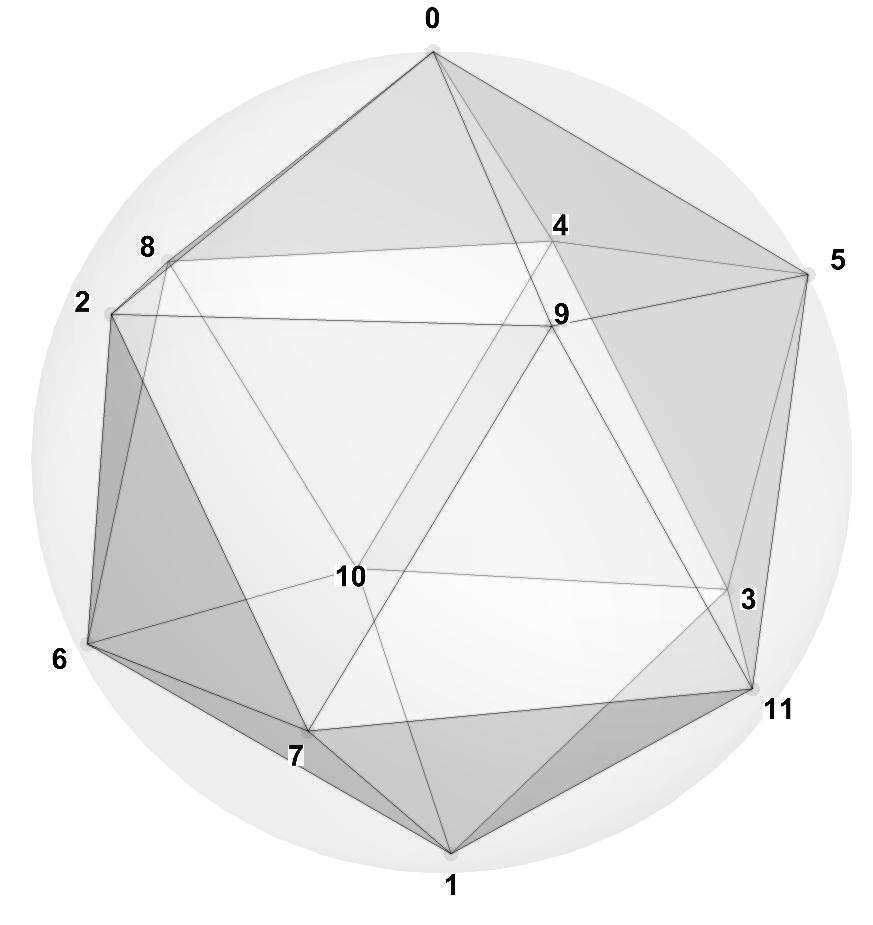
\includegraphics[width=.6\linewidth]{icosahedron}
\end{center}

\begin{itemize}[leftmargin=1.5em]
  \item \textbf{Number of scar sets:} \texttt{<1 or 2>}. 
  \item For each scar set $S_k$, fill one table per set:
\end{itemize}

\noindent\textit{Scar set} $S_{\texttt{<k>}}$:
\begin{center}
\begin{tabular}{L{3.5cm} C{2.2cm} C{2.2cm} C{2.2cm} C{3.0cm} C{3.2cm}}
\toprule
\textbf{Multiplet label} & \textbf{Energy $E$} & \textbf{Degeneracy} & \textbf{Annihilated by} & \textbf{Non-zero components (vs.\ $2^{V}$)} \\
\midrule
\texttt{<m1>} & $\pm$ \texttt{<int>} & \texttt{<deg> } &
\texttt{$\Hising$ / $\Htf$ / both} & \texttt{<\# non-zero> / $2^{\texttt{<V>}}$} \\
\bottomrule
\end{tabular}
\end{center}

\subsubsection*{Local properties (RDMs).}
\begin{center}
  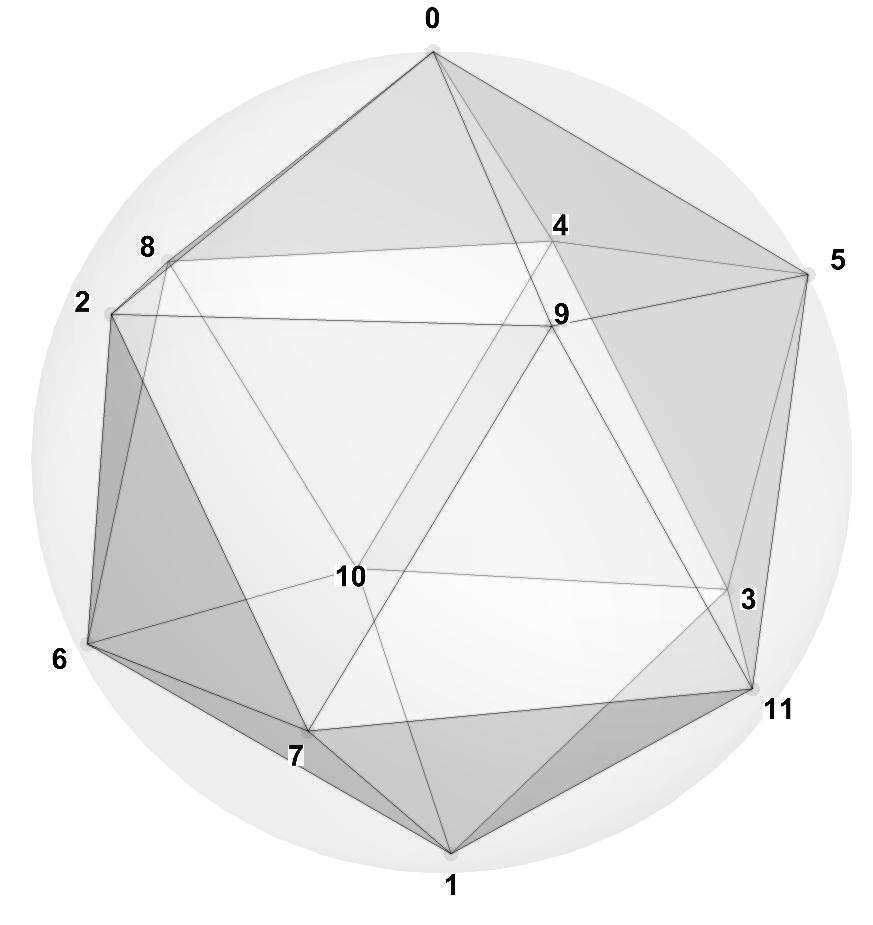
\includegraphics[width=.6\linewidth]{icosahedron}
\end{center}

\begin{itemize}[leftmargin=1.5em]
  \item \textbf{Local RDM definition:} $\rho_A=\mathrm{Tr}_{\bar A}(|\psi\rangle\langle\psi|)$ on compact subsets of $n=2,3,4,5,6$ sites, with $n < V/2$.
  \item \textbf{Compactness criterion:} \texttt{<how subsets chosen>}.
  \item \textbf{Diagnostics:} \texttt{<observables, entropies, purity, etc.>}.
\end{itemize}

% -------------------- Polyhedron Block: END --------------------

% -------------------- Polyhedron Block: START --------------------
\subsection*{Dodecahedron}

\subsubsection*{Overview and data.}
\begin{center}
  % Put your graphic at the very beginning of the subparagraph
  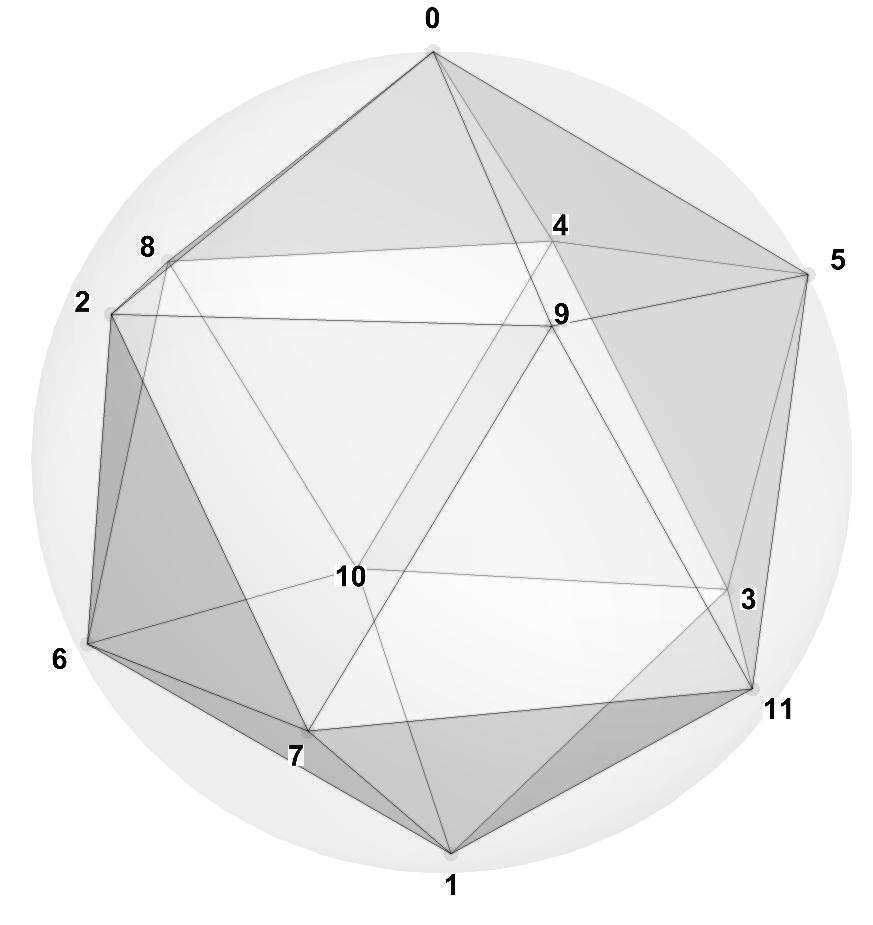
\includegraphics[width=.6\linewidth]{icosahedron}
\end{center}

\begin{itemize}[leftmargin=1.5em]
  \item \textbf{Duality / paired solid:} \texttt{<DUALITY or “self-dual”>}.
  \item \textbf{Vertices (V), Faces (F), Edges (E):} $V=\texttt{<V>}$,\; $F=\texttt{<F>}$,\; $E=\texttt{<E>}$.
  \item \textbf{Solid point group:} \texttt{<POINT-GROUP>}.\\
        \textbf{Vertex stabilizer subgroup:} \texttt{<STABILIZER>}.
  \item \textbf{Hamiltonian:} \(
        \Htot,\quad
        \dim\mathcal{H} = 2^{V}\ \text{(spin-$\tfrac12$ on each vertex).}
        \)
  \item \textbf{Eigenvalue range / normalization:} \texttt{<Specify conventions>}.
\end{itemize}

\subsubsection*{Scar structure: sets and multiplets.}
\begin{center}
  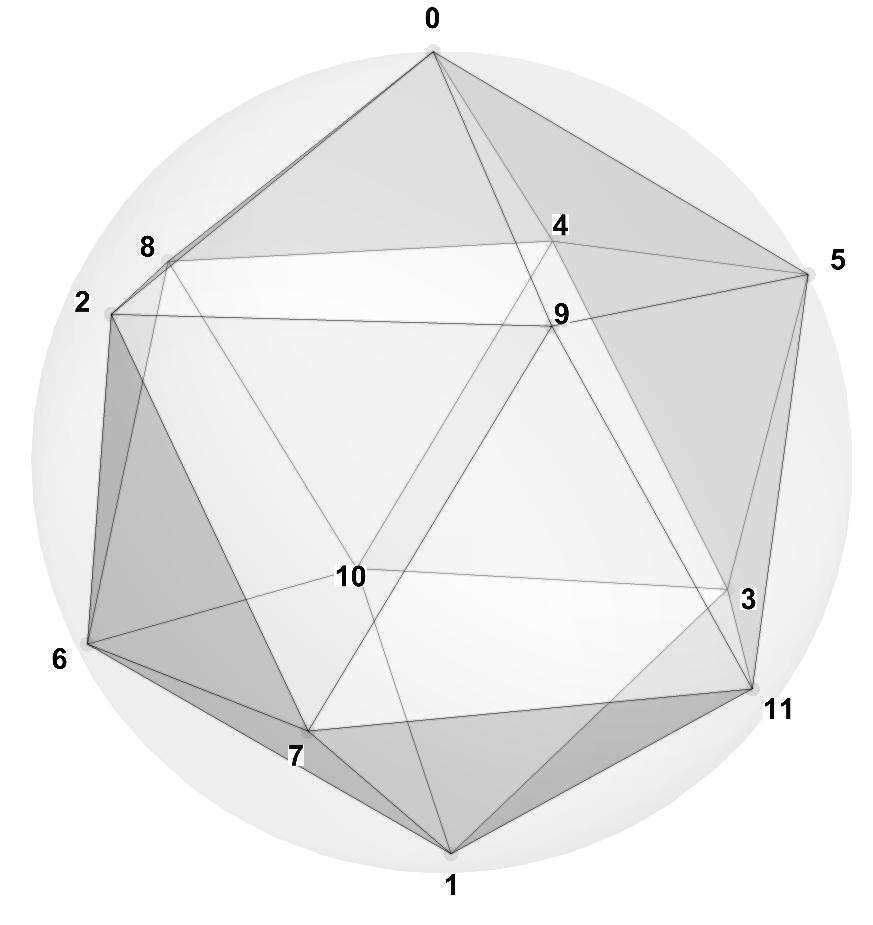
\includegraphics[width=.6\linewidth]{icosahedron}
\end{center}

\begin{itemize}[leftmargin=1.5em]
  \item \textbf{Number of scar sets:} \texttt{<1 or 2>}. 
  \item For each scar set $S_k$, fill one table per set:
\end{itemize}

\noindent\textit{Scar set} $S_{\texttt{<k>}}$:
\begin{center}
\begin{tabular}{L{3.5cm} C{2.2cm} C{2.2cm} C{2.2cm} C{3.0cm} C{3.2cm}}
\toprule
\textbf{Multiplet label} & \textbf{Energy $E$} & \textbf{Degeneracy} & \textbf{Annihilated by} & \textbf{Non-zero components (vs.\ $2^{V}$)} \\
\midrule
\texttt{<m1>} & $\pm$ \texttt{<int>} & \texttt{<deg> } &
\texttt{$\Hising$ / $\Htf$ / both} & \texttt{<\# non-zero> / $2^{\texttt{<V>}}$} \\
\bottomrule
\end{tabular}
\end{center}

\subsubsection*{Local properties (RDMs).}
\begin{center}
  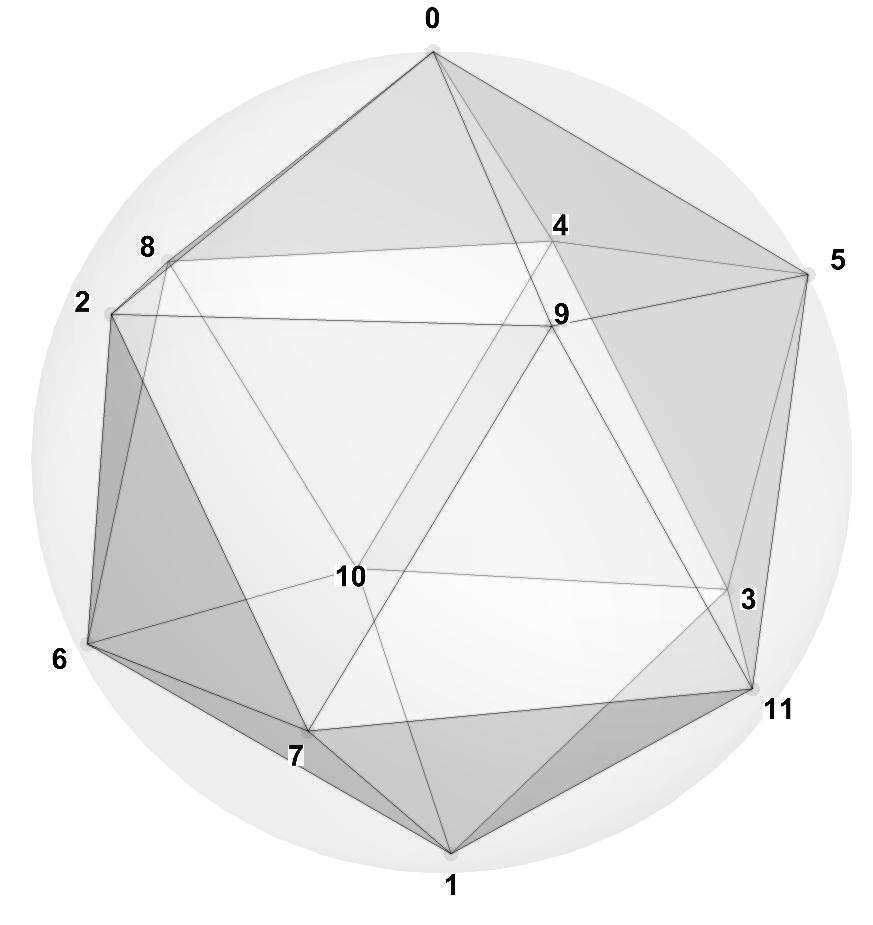
\includegraphics[width=.6\linewidth]{icosahedron}
\end{center}

\begin{itemize}[leftmargin=1.5em]
  \item \textbf{Local RDM definition:} $\rho_A=\mathrm{Tr}_{\bar A}(|\psi\rangle\langle\psi|)$ on compact subsets of $n=2,3,4,5,6$ sites, with $n < V/2$.
  \item \textbf{Compactness criterion:} \texttt{<how subsets chosen>}.
  \item \textbf{Diagnostics:} \texttt{<observables, entropies, purity, etc.>}.
\end{itemize}

% -------------------- Polyhedron Block: END --------------------

\section*{Archimedean Solids}
% ============================================================
% REPEAT THE BLOCK BELOW FOR EACH POLYHEDRON
% ============================================================

% -------------------- Polyhedron Block: START --------------------
\subsection*{Truncated Tetrahedron}

\subsubsection*{Overview and data.}
\begin{center}
  % Put your graphic at the very beginning of the subparagraph
  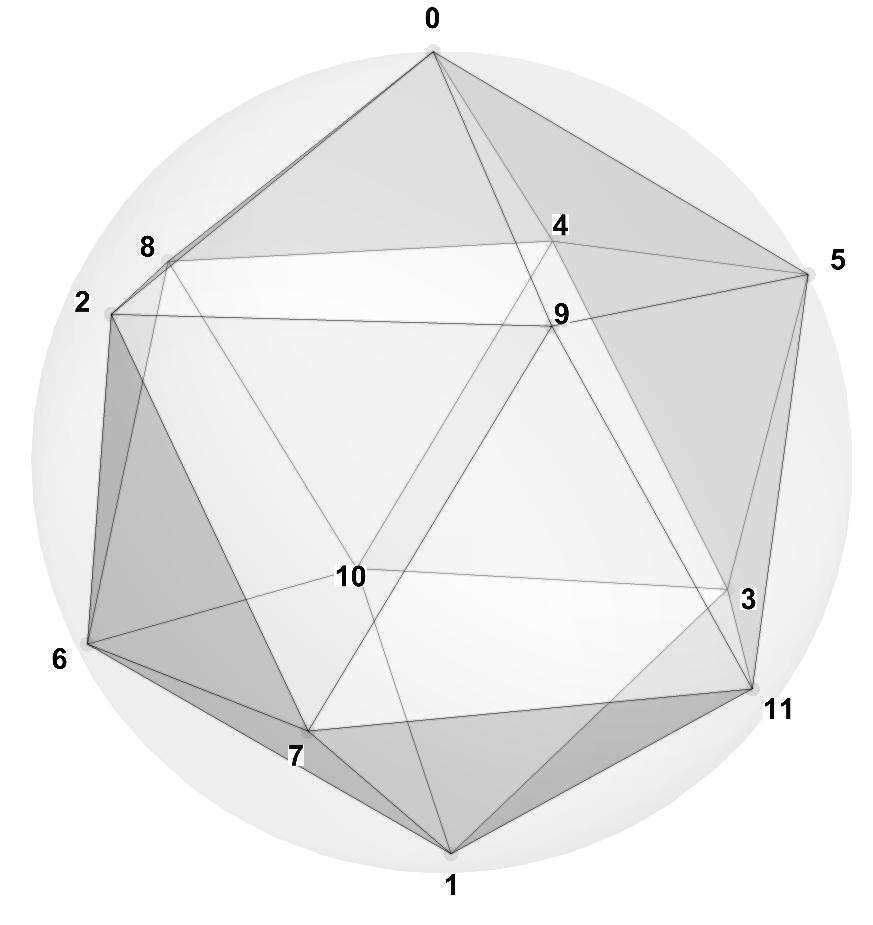
\includegraphics[width=.6\linewidth]{icosahedron}
\end{center}

\begin{itemize}[leftmargin=1.5em]
  \item \textbf{Duality / paired solid:} \texttt{<DUALITY or “self-dual”>}.
  \item \textbf{Vertices (V), Faces (F), Edges (E):} $V=\texttt{<V>}$,\; $F=\texttt{<F>}$,\; $E=\texttt{<E>}$.
  \item \textbf{Solid point group:} \texttt{<POINT-GROUP>}.\\
        \textbf{Vertex stabilizer subgroup:} \texttt{<STABILIZER>}.
  \item \textbf{Hamiltonian:} \(
        \Htot,\quad
        \dim\mathcal{H} = 2^{V}\ \text{(spin-$\tfrac12$ on each vertex).}
        \)
  \item \textbf{Eigenvalue range / normalization:} \texttt{<Specify conventions>}.
\end{itemize}

\subsubsection*{Scar structure: sets and multiplets.}
\begin{center}
  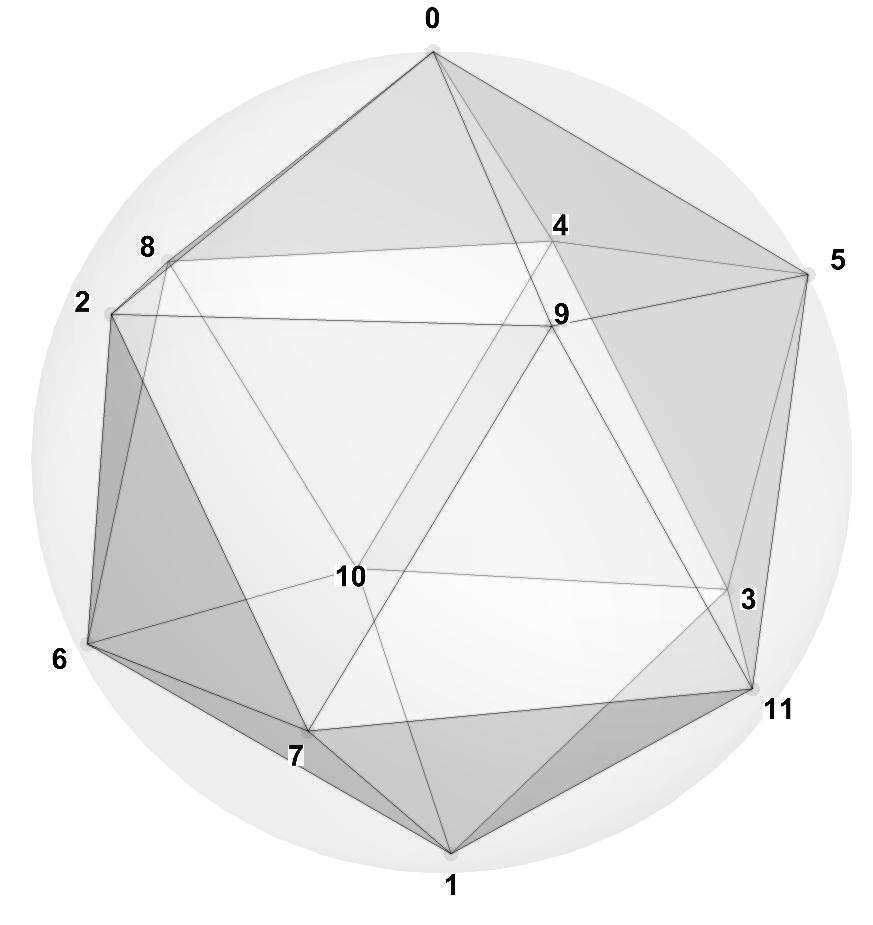
\includegraphics[width=.6\linewidth]{icosahedron}
\end{center}

\begin{itemize}[leftmargin=1.5em]
  \item \textbf{Number of scar sets:} \texttt{<1 or 2>}. 
  \item For each scar set $S_k$, fill one table per set:
\end{itemize}

\noindent\textit{Scar set} $S_{\texttt{<k>}}$:
\begin{center}
\begin{tabular}{L{3.5cm} C{2.2cm} C{2.2cm} C{2.2cm} C{3.0cm} C{3.2cm}}
\toprule
\textbf{Multiplet label} & \textbf{Energy $E$}  & \textbf{Degeneracy} & \textbf{Annihilated by} & \textbf{Non-zero components (vs.\ $2^{V}$)} \\
\midrule
\texttt{<m1>} & $\pm$ \texttt{<int>} & \texttt{<deg> } &
\texttt{$\Hising$ / $\Htf$ / both} & \texttt{<\# non-zero> / $2^{\texttt{<V>}}$} \\
\bottomrule
\end{tabular}
\end{center}

\subsubsection*{Local properties (RDMs).}
\begin{center}
  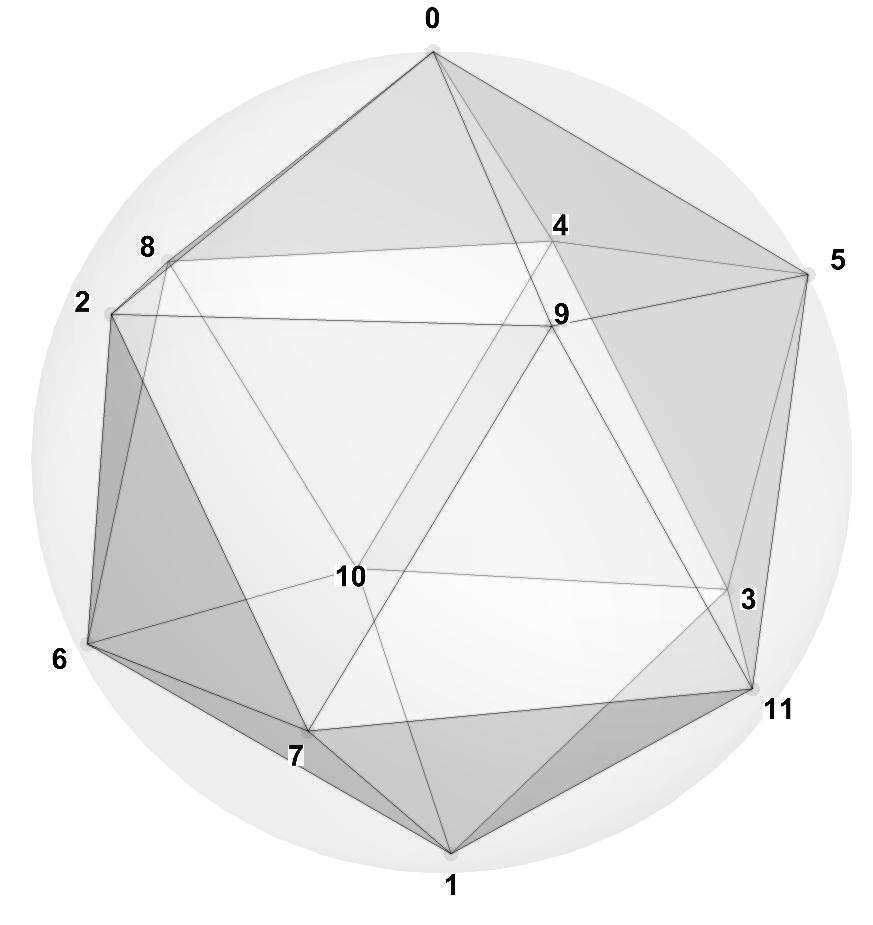
\includegraphics[width=.6\linewidth]{icosahedron}
\end{center}

\begin{itemize}[leftmargin=1.5em]
  \item \textbf{Local RDM definition:} $\rho_A=\mathrm{Tr}_{\bar A}(|\psi\rangle\langle\psi|)$ on compact subsets of $n=2,3,4,5,6$ sites, with $n < V/2$.
  \item \textbf{Compactness criterion:} \texttt{<how subsets chosen>}.
  \item \textbf{Diagnostics:} \texttt{<observables, entropies, purity, etc.>}.
\end{itemize}

% -------------------- Polyhedron Block: END --------------------

% -------------------- Polyhedron Block: START --------------------
\subsection*{Cuboctahedron}

\subsubsection*{Overview and data.}
\begin{center}
  % Put your graphic at the very beginning of the subparagraph
  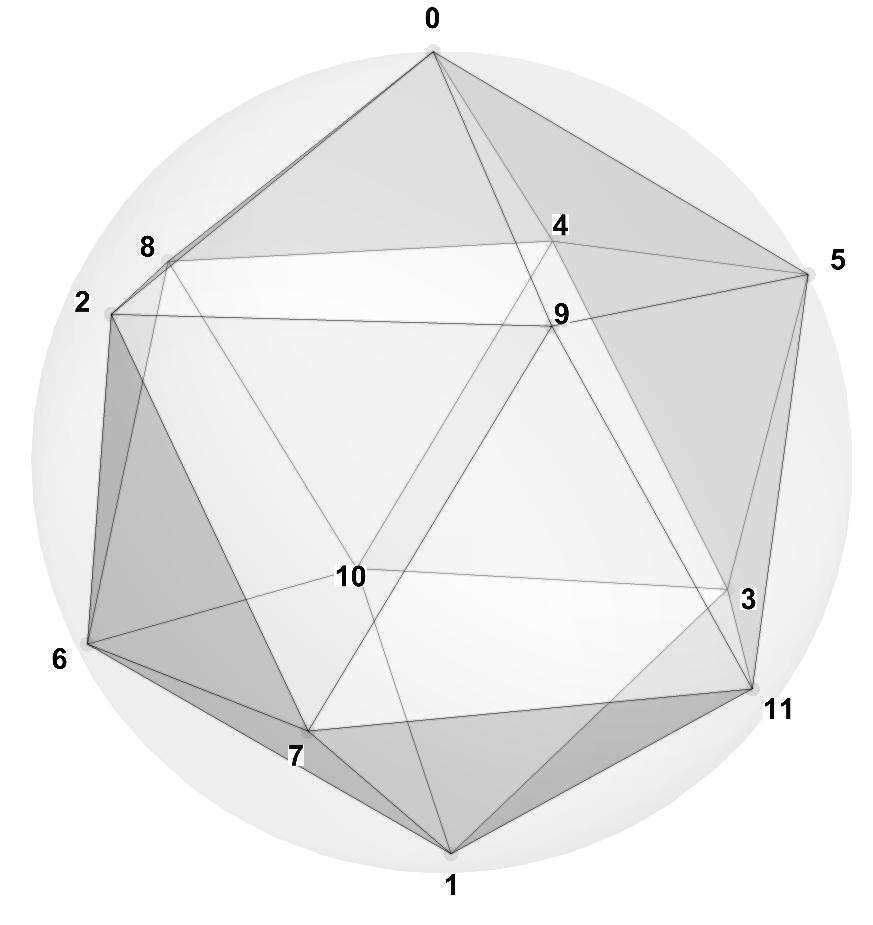
\includegraphics[width=.6\linewidth]{icosahedron}
\end{center}

\begin{itemize}[leftmargin=1.5em]
  \item \textbf{Duality / paired solid:} \texttt{<DUALITY or “self-dual”>}.
  \item \textbf{Vertices (V), Faces (F), Edges (E):} $V=\texttt{<V>}$,\; $F=\texttt{<F>}$,\; $E=\texttt{<E>}$.
  \item \textbf{Solid point group:} \texttt{<POINT-GROUP>}.\\
        \textbf{Vertex stabilizer subgroup:} \texttt{<STABILIZER>}.
  \item \textbf{Hamiltonian:} \(
        \Htot,\quad
        \dim\mathcal{H} = 2^{V}\ \text{(spin-$\tfrac12$ on each vertex).}
        \)
  \item \textbf{Eigenvalue range / normalization:} \texttt{<Specify conventions>}.
\end{itemize}

\subsubsection*{Scar structure: sets and multiplets.}
\begin{center}
  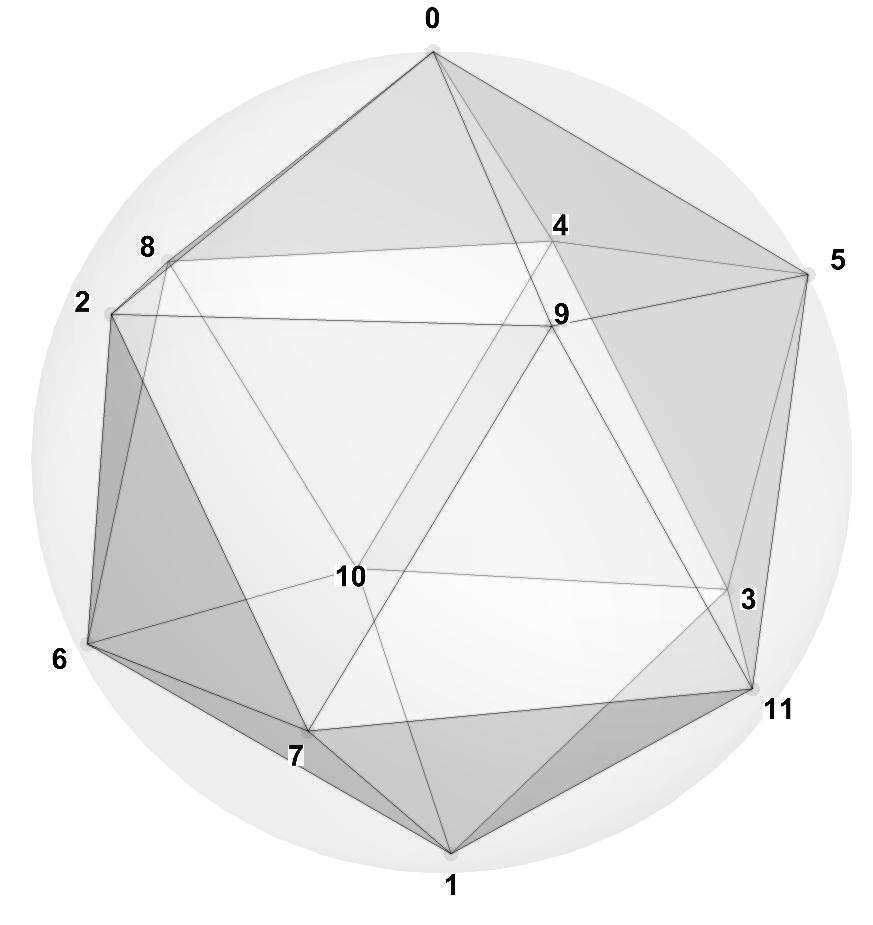
\includegraphics[width=.6\linewidth]{icosahedron}
\end{center}

\begin{itemize}[leftmargin=1.5em]
  \item \textbf{Number of scar sets:} \texttt{<1 or 2>}. 
  \item For each scar set $S_k$, fill one table per set:
\end{itemize}

\noindent\textit{Scar set} $S_{\texttt{<k>}}$:
\begin{center}
\begin{tabular}{L{3.5cm} C{2.2cm} C{2.2cm} C{2.2cm} C{3.0cm} C{3.2cm}}
\toprule
\textbf{Multiplet label} & \textbf{Energy $E$} & \textbf{Degeneracy} & \textbf{Annihilated by} & \textbf{Non-zero components (vs.\ $2^{V}$)} \\
\midrule
\texttt{<m1>} & $\pm$ \texttt{<int>} & \texttt{<deg> } &
\texttt{$\Hising$ / $\Htf$ / both} & \texttt{<\# non-zero> / $2^{\texttt{<V>}}$} \\
\bottomrule
\end{tabular}
\end{center}

\subsubsection*{Local properties (RDMs).}
\begin{center}
  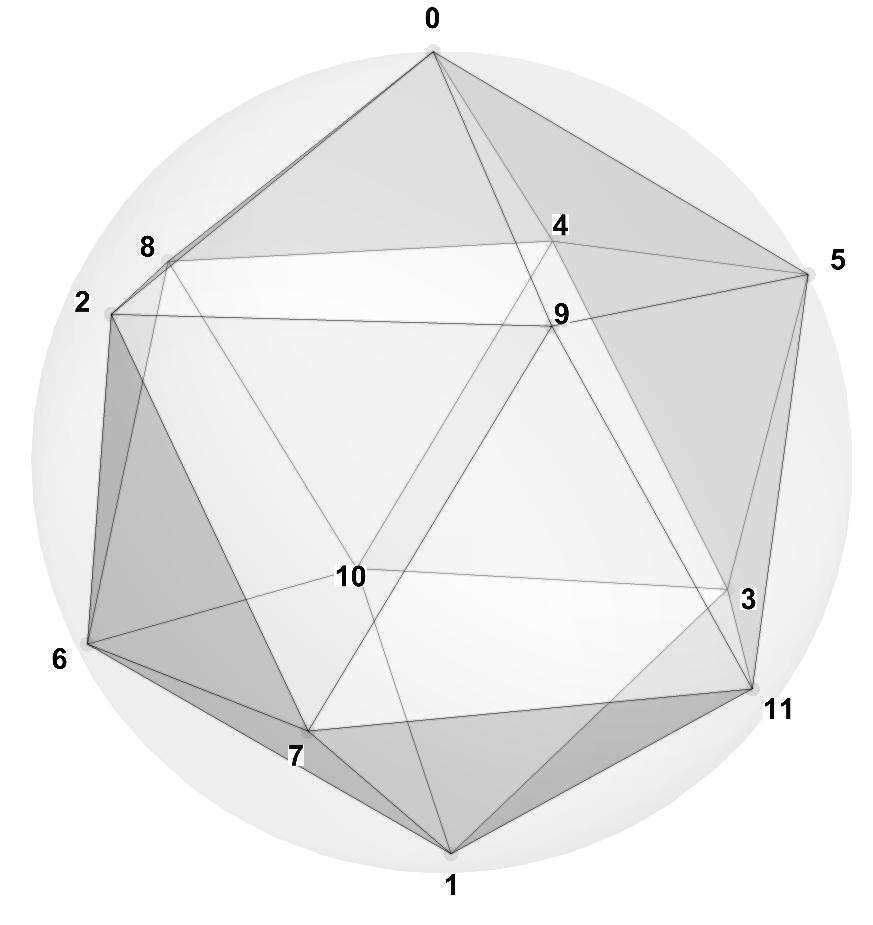
\includegraphics[width=.6\linewidth]{icosahedron}
\end{center}

\begin{itemize}[leftmargin=1.5em]
  \item \textbf{Local RDM definition:} $\rho_A=\mathrm{Tr}_{\bar A}(|\psi\rangle\langle\psi|)$ on compact subsets of $n=2,3,4,5,6$ sites, with $n < V/2$.
  \item \textbf{Compactness criterion:} \texttt{<how subsets chosen>}.
  \item \textbf{Diagnostics:} \texttt{<observables, entropies, purity, etc.>}.
\end{itemize}

% -------------------- Polyhedron Block: END --------------------



\end{document}
